\documentclass[16pt]{mythesis}
\usepackage{booktabs}
\usepackage{float}
\usepackage{tikz}
\usepackage{tabto} 
\usepackage{minted}
\setminted{
    linenos=true,     % Add line numbers
    breaklines=true,  % Wrap long lines
    frame=lines,      % Add lines above and below the code
    fontsize=\footnotesize
}
\def\checkmark{\tikz\fill[scale=0.4](0,.35) -- (.25,0) -- (1,.7) -- (.25,.15) -- cycle;}  


\newcommand{\mynote}[3]{
    \fbox{\bfseries\sffamily\scriptsize#1}
    {\small$\blacktriangleright$\textsf{\emph{\color{#3}{#2}}}$\blacktriangleleft$}}
\newcommand{\yb}[1]{\mynote{Yahia}{#1}{red}}
%\usepackage{arabtex}

% Packages you intend to use
% ..

% For example, if you want to render 
% the document in a different font you can
% use something like: 

%\usepackage{gentium}
%\usepackage{txfonts}
%\usepackage[sfdefault]{roboto}


% Or maybe you want clickable references in your thesis:
\usepackage{hyperref}
\usepackage[T1]{fontenc}
\usepackage[utf8]{inputenc}
\usepackage{lmodern}
\usepackage[a4paper, top=2.5cm, bottom=2.5cm, left=3cm, right=2.5cm]{geometry}
\usepackage{graphicx}
\usepackage{array}
\usepackage{tabularx}
\usepackage{longtable}
\usepackage{listings}
\usepackage{xcolor}
\usepackage{amsmath}
\usepackage{fancyhdr}
\usepackage{titlesec}
\usepackage{hyperref}
\usepackage{caption}
\usepackage{setspace}
\usepackage{emptypage}
\usepackage{tocloft}
\input{preamble/bib-setup}
%% Below are a bunch of details for formatting your undergraduate thesis.
%% Make sure to fill each of these out.

% The title of your thesis (If your title is very large, consider prepending
% it with the \Large command
\title{\bfseries Bachelor Project Title}

% The degree
\thesisDegree{Bachelor}

% The programme
\thesisProgramme{Electrical and Electronic Engineering}

% The school name
\thesisSchool{Institute of Electrical and Electronic Engineering}

% The university
\thesisUniversity{M'Hamed Bougara University of Boumerdes}

% The date (which is shown last, you can just put a year in here):
\date{June 2025}

% The authors
\author{Student name 1\\Student name 2\\Student name 3}

% Degree already declared above
% \thesisDegree{}

% Submission date
\thesisSubmissionDate{June 2025}

% Supervisor details
\thesisSupervisor{supervisor name}

% Optional: header/footer settings
% \thesisTurnOffHF



\begin{document}
\maketitle

% Input anything that can go before the acknowledgements 

%\input{chapters/blank-pages.tex}

% Then the acknowledgements
\begin{Dedications}
\paragraph{}

This thesis is dedicated to our lovely parents for their endless support and encouragement and to our dear brothers. We further extend our dedication to all members of the family. 
\paragraph{}
We dedicate this work also without exception to all our friends, colleagues, and teachers. 
\paragraph{}
Last and not least, I dedicate our work to everyone who has taught, encouraged, and advised us during all our studies. 

\end{Dedications}

\begin{Acknowledgments}

                              






\paragraph{}
%This thesis is dedicated to my lovely parents for their endless support and encouragement, to my dear brothers. I further extend my dedication to all members of Touzout's family. 
%\paragraph{}
%I dedicate this work also without exception to all my friends, colleagues, and my teachers. 
%\paragraph{}
%Last and not least, I dedicate my PhD to everyone who has taught, encouraged, and advised me during all my studies. 


First and foremost, all praise and thanks giving to Allah the most powerful and most merciful who gave me the ability and patience to accomplish the work presented. 
\paragraph{}

\end{Acknowledgments}




\begin{abstract}
\paragraph{}
This project presents a customizable LaTeX template designed to streamline the creation of academic documents such as theses, reports, or research papers. 
effort. . 
\paragraph{}
The template adheres to standardized formatting guidelines and includes predefined sections, citation styles, and typographic elements to ensure consistency and professionalism. It serves as a practical starting point for students, researchers, and professionals seeking to produce well-structured documents with minimal formatting 

\begin{itemize}
\item this is item 1
\item this is item 2 \cite{example_reference1}.
\end{itemize}

%\paragraph{}
%\begin{keywords}

%\end{keywords}
\end{abstract} 






%\input{chapters/abstractAr}
% Print out the table of tables and table of figures and
% tell the template we're about to start the body of the
% thesis.

\thesisTables


\begin{Abbreviations}


CISC    \hfill Complex Instruction Set Computer     \\ 
RISC    \hfill Reduced Instruction Set Computer   \\                   
ISA    \hfill Instruction Set Architecture   \\                   
RV32I  \hfill RISC-V 32-bit Base Integer ISA    \\
GCC    \hfill GNU Compiler Collection \\
NOP    \hfill No Operation     \\


\end{Abbreviations} 
%\thesisBodyStart

% start of thesis body
% ---------------------------
%\Include {introduction}






% Print out the table of tables and table of figures and
% tell the template we're about to start the body of the
% thesis.
%\thesisTab  
\thesisBodyStart

% start of thesis body
% ---------------------------
%\Include {introduction}

\chapter{Introduction}
%\begin{}
\paragraph{ }
A processor is a specialized digital circuit designed to execute instructions, perform mathematical and logical calculations, and control data flow within a computer system. Over the past decades, microprocessors have not only become a defining trend in the technology industry but have fundamentally reshaped it. As a result, studying and advancing processor design remains a priority for both industry and academia.
\paragraph{}
RISC-V (Reduced Instruction Set Computer - Five) is an open-standard instruction set architecture (ISA) developed in 2010 at UC Berkeley by Krste Asanović, Andrew Waterman, and Yunsup Lee under the supervision of David Patterson. What makes it unique is its open-standard nature, allowing users to adopt it freely and even modify it, fostering rapid adoption across both academic and commercial domains. Additionally, its adherence to the RISC philosophy makes it not only easier to design and implement but also inherently energy efficient.
\paragraph{}
This project presents BigDCore (Big Dream Core), a pipelined 32-bit processor implementing the full RV32I Base Integer ISA, described in VHDL and targeting simulation-based verification. RV32I was chosen as the target ISA for its completeness as a base integer instruction set while remaining tractable for a single academic project. Testing is conducted using the industry-standard simulation tool ModelSim, and future work includes the privileged architecture to enable an operating system to run on the processor.


% Literature review / Background / Related work
\chapter{RISC-V Theoretical Background \& System Architecture}

\section{Introduction}
\paragraph{}

This chapter presents the theoretical foundations underlying the design and implementation of BigDCore. It covers three principal areas: the RISC-V instruction set architecture, fundamental processor design concepts, and an overview of existing RISC-V soft-core implementations. Together, these establish the academic and technical context within which this project is situated.

\section{RISC-V Instruction Set Architecture}
\subsection{History and Origin}

The RISC-V ISA was conceived in 2010 at the University of California, Berkeley, as part of the fifth generation of RISC research projects conducted at the institution. It was developed by Krste Asanović, Andrew Waterman, and Yunsup Lee under the supervision of David Patterson, one of the pioneers of the original RISC architecture. Unlike previous ISA efforts, RISC-V was designed from the outset to be open, stable, and free from proprietary constraints, making it suitable for both academic research and commercial deployment. In 2015, the RISC-V Foundation was established to govern the specification, which was later transferred to RISC-V International in 2020 to ensure its long-term neutrality and global accessibility.
\subsection{Design Philosophy}

RISC-V adheres to the core principles of Reduced Instruction Set Computing. Its design philosophy prioritizes simplicity, regularity, and extensibility. The base ISA is intentionally kept minimal, containing only the instructions necessary for general-purpose computation, while optional standard extensions allow the ISA to be tailored for specific application domains such as floating-point arithmetic, atomic operations, compressed instructions, and vector processing. This modularity ensures that a processor designer can implement only the subset relevant to their use case without carrying the overhead of unused hardware.

A key distinguishing characteristic of RISC-V is its fixed 32-bit instruction width in the base integer ISA, which simplifies instruction fetch and decode logic. All instructions follow a small number of regular formats, and frequently used fields such as the source and destination register indices appear at fixed bit positions across all formats, reducing decoder complexity.
\subsection{RV32I Instruction Formats}
The RV32I base integer ISA defines six instruction formats, each encoding a different combination of operands and immediate values while maintaining a fixed 32-bit instruction width.
\begin{figure}[h!]
    \centering
    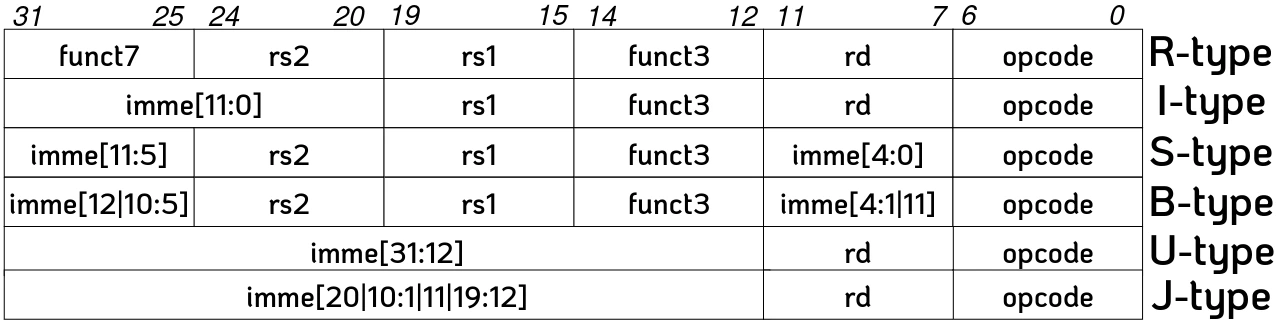
\includegraphics[scale=0.3]{Figures/Chapter 2/Instruction-Formats-RV32I.png}
    \caption{RV32I Instruction Formats}
    \label{fig:RV32I Instruction Formats}
\end{figure}

The \textbf{R-type} format is used for register-to-register arithmetic and logical operations. It encodes two source registers (rs1, rs2) and one destination register (rd), along with a 7-bit opcode, a 3-bit funct3 field, and a 7-bit funct7 field that together uniquely identify the operation.

The \textbf{I-type} format is used for immediate arithmetic operations, load instructions, and environment calls. It encodes one source register (rs1), one destination register (rd), and a 12-bit signed immediate value.

The \textbf{S-type} format is used exclusively for store instructions. It encodes two source registers and a 12-bit signed immediate that is split across two non-contiguous fields in the instruction word, a deliberate design choice to keep the register fields at fixed positions.

The \textbf{B-type} format is used for conditional branch instructions. It encodes two source registers and a 13-bit signed immediate representing a PC-relative branch offset. Like the S-type, the immediate bits are shuffled to preserve fixed register field positions.

The \textbf{U-type} format is used for instructions that operate on upper immediates, namely LUI (Load Upper Immediate) and AUIPC (Add Upper Immediate to PC). It encodes a 20-bit immediate and a destination register.

The \textbf{J-type} format is used exclusively by the JAL (Jump and Link) instruction. It encodes a 21-bit PC-relative jump offset and a destination register that receives the return address.
\subsection{Processor Design Concepts}
\subsubsection{Von Neumann vs. Harvard Architecture}
Two fundamental memory architectures underpin modern processor design. The von Neumann architecture, proposed by John von Neumann in 1945, uses a single shared memory space and a single bus to carry both instructions and data. While this simplifies the memory system and allows flexible allocation of memory between code and data, it introduces a structural bottleneck known as the von Neumann bottleneck: the processor cannot fetch an instruction and access data simultaneously, limiting throughput.

The Harvard architecture addresses this limitation by providing physically separate memories and buses for instructions and data. This allows simultaneous access to both, eliminating the structural hazard present in von Neumann designs and improving pipeline throughput. The cost is a less flexible memory system, as instruction and data memory cannot share capacity.

A Modified Harvard architecture is a practical compromise widely adopted in modern processors. It maintains separate instruction and data caches at the first level, providing the performance benefits of Harvard architecture, while using a unified main memory accessible by both, preserving the flexibility of von Neumann memory management.

BigDCore adopts a Harvard architecture with fully separate instruction and data memories. This design decision directly supports the five-stage pipeline by ensuring that instruction fetch and data memory access never contend for the same resource.
\subsubsection{Single-Cycle vs. Pipelined Execution}
A single-cycle processor completes the execution of one instruction per clock cycle by routing it through all functional units in a single pass. While conceptually simple, this approach requires the clock period to be long enough to accommodate the slowest possible instruction, resulting in poor clock frequency and underutilization of hardware during the execution of faster instructions.

A pipelined processor overlaps the execution of multiple instructions by dividing the datapath into discrete stages, each handling one phase of execution. While an individual instruction still takes multiple cycles to complete, the throughput approaches one instruction per cycle under ideal conditions, and the clock period is determined by the slowest pipeline stage rather than the slowest instruction. This trade-off introduces pipeline hazards — structural, data, and control hazards — which must be managed through stalling, forwarding, and flushing mechanisms.

BigDCore implements a classical five-stage pipeline comprising the Instruction Fetch (IF), Instruction Decode (ID), Execute (EX), Memory Access (MEM), and Write-Back (WB) stages. A hazard detection unit manages data hazards through stalling and forwarding, and control hazards arising from branch instructions are resolved through pipeline flushing.

\section{Top-Level Architecture}
At the highest level of abstraction, RV32ICore is composed of two primary units: the Datapath and the Control Unit, along with a dedicated Hazard Unit that operates across pipeline stages.

\textbf{The Datapath} is responsible for processing and routing data throughout the processor. Its inputs include control signals generated by the Control Unit, instructions fetched from instruction memory, and data read from data memory. Its outputs include the Program Counter (PC) supplied to instruction memory, data written to data memory, and status information such as instruction fields and condition flags fed back to the Control Unit.

\textbf{The Control Unit} is responsible for managing the correct execution of instructions by interpreting instruction fields and generating the appropriate control signals for each pipeline stage. Its inputs are the opcode (bits [6:0]), Funct3 (bits [14:12]), and Funct7 bit 30, along with the processor clock and reset. Its outputs are the set of control signals that govern the behavior of multiplexers, the register file, the ALU, and the data memory throughout the datapath.

\textbf{The Hazard Unit} monitors the pipeline state and intervenes when hazard conditions are detected. It generates stall and flush signals to preserve correct program execution in the presence of data dependencies and control flow changes. Its operation is described in detail in Section 3.9.
\begin{figure}[h!]
	\centering
	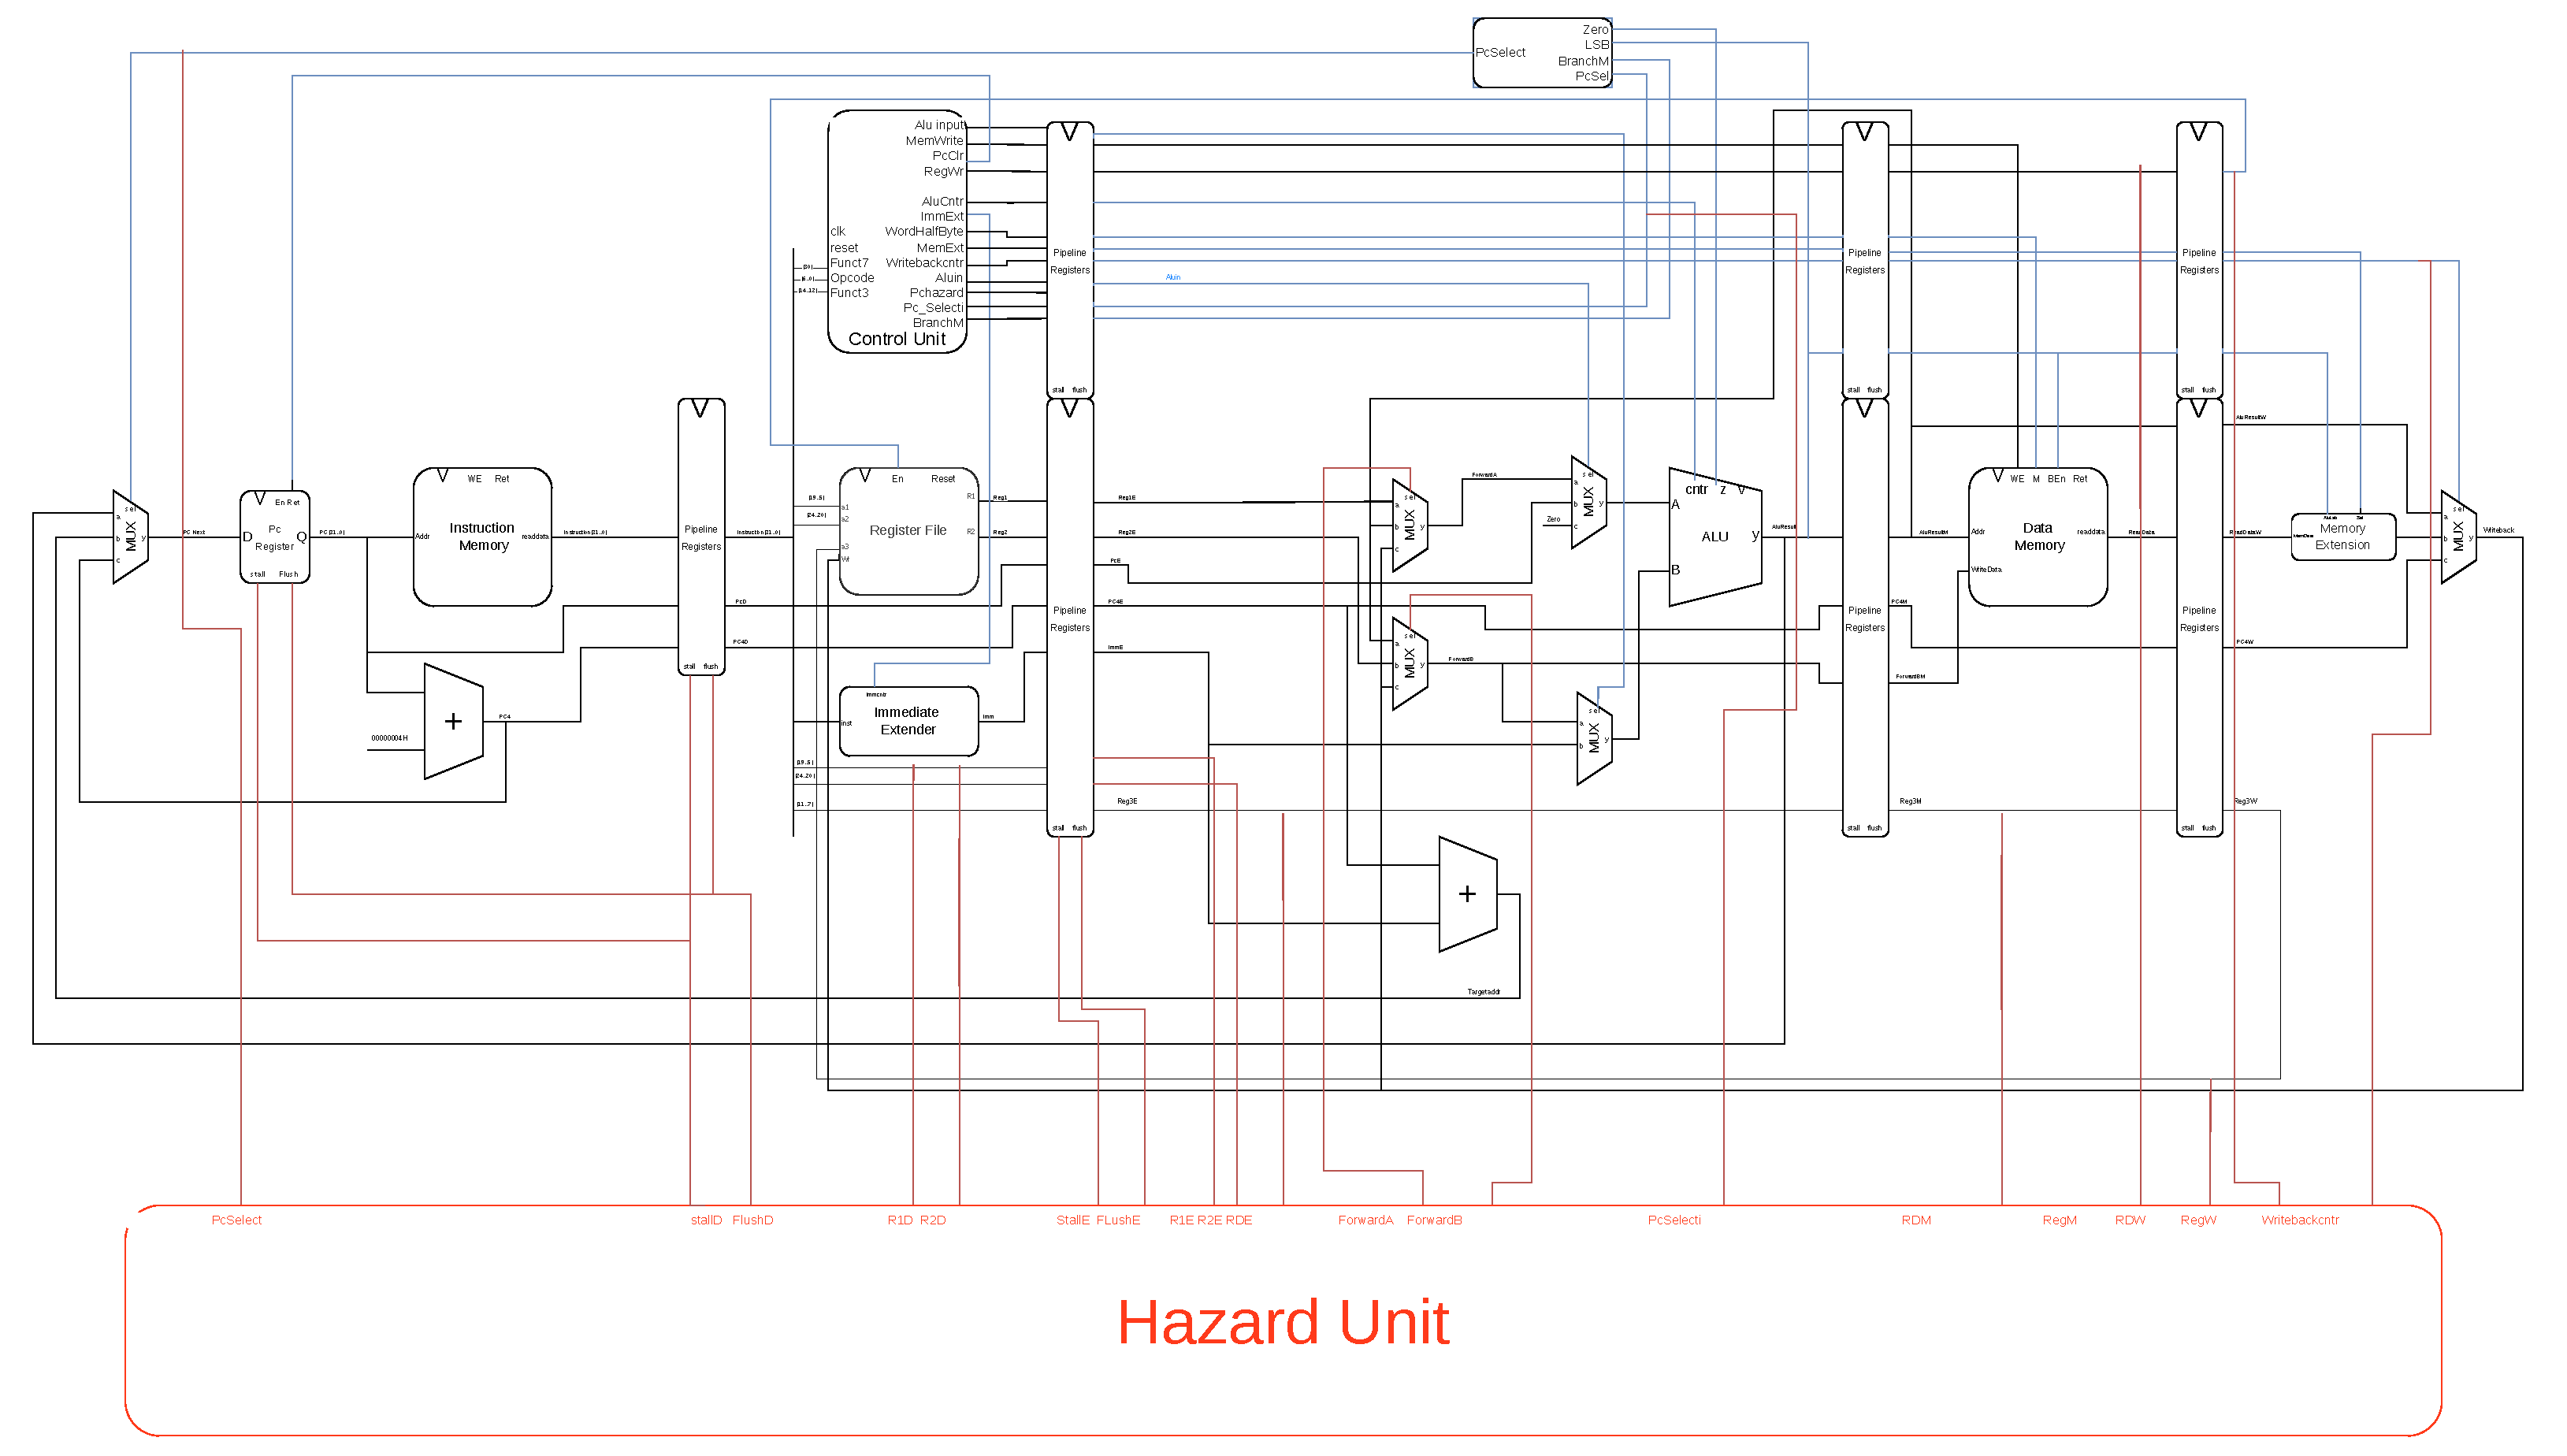
\includegraphics[scale=0.3]{Figures/Chapter 3/Top Level.pdf}
	\caption{RV32ICore Top-Level Architecture}
	\label{fig: RV32ICore Top-Level Architecture}
\end{figure}
\section{Pipeline Overview}
RV32ICore implements a classical five-stage pipeline. Pipelining allows multiple instructions to be in different stages of execution simultaneously, improving throughput by overlapping work across stages. The five stages are:

\begin{itemize}
	\item \textbf{IF} — Instruction Fetch
	\item \textbf{ID} — Instruction Decode
	\item \textbf{EX} — Execute
	\item \textbf{MEM} — Memory Access
	\item \textbf{WB} — Write-Back
\end{itemize}

Each stage is separated from the next by a pipeline register that captures the outputs of the current stage and holds them stable for the following stage on the next clock edge. All pipeline registers share the same clock as the rest of the processor and are controlled by two signals: a synchronous reset that clears the register to zero, and a NOP insertion signal that loads a harmless no-operation instruction into the register without clearing its other fields, used during flush operations.
\section{Instruction Fetch (IF) Stage}
The Instruction Fetch stage is responsible for retrieving the current instruction from instruction memory and advancing the Program Counter

The PC is stored in a dedicated register that updates on every rising clock edge under normal operation. Its value is used directly as the address supplied to the instruction memory, which responds combinationally with the 32-bit instruction word stored at that address.

A dedicated adder computes PC+4, representing the address of the next sequential instruction. This value is carried forward through the pipeline and is used in the Write-Back stage as the return address for jump instructions.

On a taken branch, the PC is updated to the branch target address computed in the Execute stage in the same cycle that the flush signal is issued. Under normal sequential execution, the PC is updated to PC+4.

The instruction memory is separate from the data memory, consistent with the Harvard architecture adopted by RV32ICore. This ensures that instruction fetch never contends with data memory access, eliminating structural hazards between the IF and MEM stages.
\begin{figure}[h!]
	\centering
	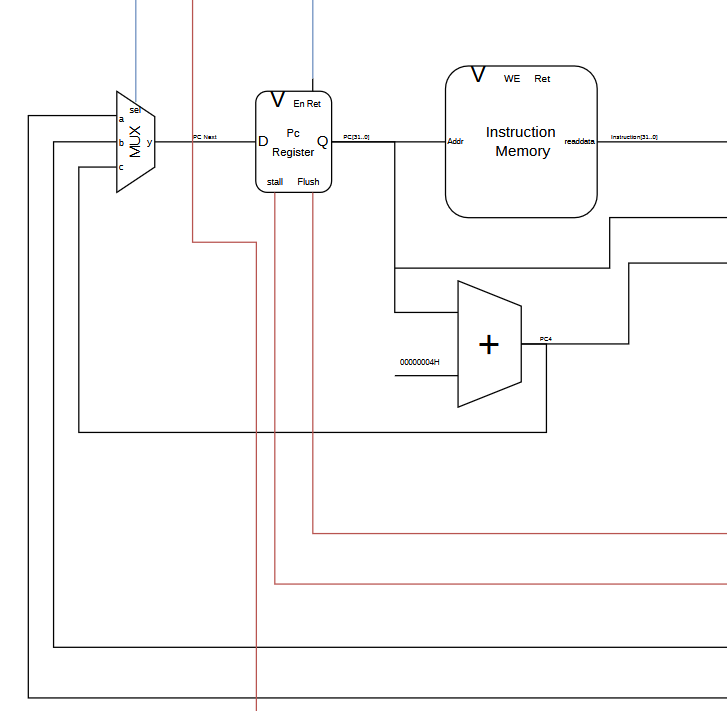
\includegraphics[scale=0.3]{Figures/Chapter 3/IF Stage.png}
	\caption{RV32ICore IF Stage}
	\label{fig: RV32ICore IF Stage}
\end{figure}
\section{Instruction Decode (ID) Stage}
The Instruction Decode stage deconstructs the fetched instruction and prepares the operands and control signals required for execution.

The 32-bit instruction word is partitioned into its constituent fields according to the RV32I specification. The source register addresses rs1 and rs2 are located at bits [19:15] and [24:20] respectively, and the destination register address rd is located at bits [11:7]. These addresses are wired directly to the read ports of the register file, which responds combinationally with the contents of the addressed registers. Register x0 is hardwired to zero; any read of x0 returns zero and any write to x0 is silently discarded.

An Immediate Extension unit receives the full 32-bit instruction word and produces a 32-bit sign-extended immediate value. The extension logic selects the appropriate immediate format — I, S, B, U, or J — based on the opcode, and assembles the immediate from the relevant instruction bits according to the RV32I encoding specification.

The opcode (bits [6:0]), Funct3 (bits [14:12]), and Funct7 bit 30 are forwarded to the Control Unit, which decodes them and generates the full set of control signals for the instruction. These control signals are stored in the ID/EX pipeline register alongside the register data and immediate value and propagate through the pipeline with the instruction.
\begin{figure}[h!]
	\centering
	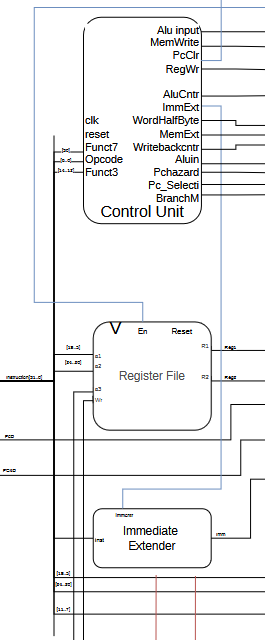
\includegraphics[scale=0.3]{Figures/Chapter 3/ID Stage.png}
	\caption{RV32ICore ID Stage}
	\label{fig: RV32ICore ID Stage}
\end{figure}
\section{Execute (EX) Stage}
The Execute stage performs the arithmetic, logical, or address computation required by the current instruction. It is the most complex stage of the datapath, containing the ALU, two input multiplexers, a branch adder, and the forwarding multiplexer logic.
\subsection{ALU Input Selection}
Two multiplexers select the operands presented to the ALU inputs.

\textbf{MuxX3} selects ALU input A from three possible sources: the value of register rs1, the current PC (used by AUIPC), or zero (used by LUI, which adds the upper immediate to zero so that the ALU result path is reused without requiring dedicated hardware). The selection is governed by a control signal generated by the Control Unit.

\textbf{MuxX2} selects ALU input B from two possible sources: the value of register rs2 (for register-to-register instructions) or the sign-extended immediate (for immediate-type instructions). The selection is governed by a corresponding control signal.

\subsection{ALU Operation}
The ALU receives the two selected operands and performs the operation specified by the ALU control signal, which is derived from the opcode, Funct3, and Funct7 fields decoded in the Control Unit. Supported operations include addition, subtraction, bitwise AND, OR, and XOR, logical and arithmetic shift, and signed and unsigned comparison. The ALU produces a 32-bit result and a zero flag used for branch condition evaluation.
\subsection{Branch Address Computation}
A dedicated adder computes the branch target address by summing the PC value carried from the IF stage with the sign-extended immediate. This target address is passed to the PC register when a branch is taken.
\subsection{Branch Resolution}
Branch conditions are evaluated in the Execute stage. When a branch is taken, the Hazard Unit issues a flush signal that inserts NOP instructions into the IF/ID and ID/EX pipeline registers in the same cycle that the PC is updated to the branch target. This discards the two incorrectly fetched instructions that entered the pipeline after the branch. No branch prediction is employed; the pipeline always flushes on a taken branch.
\begin{figure}[h!]
	\centering
	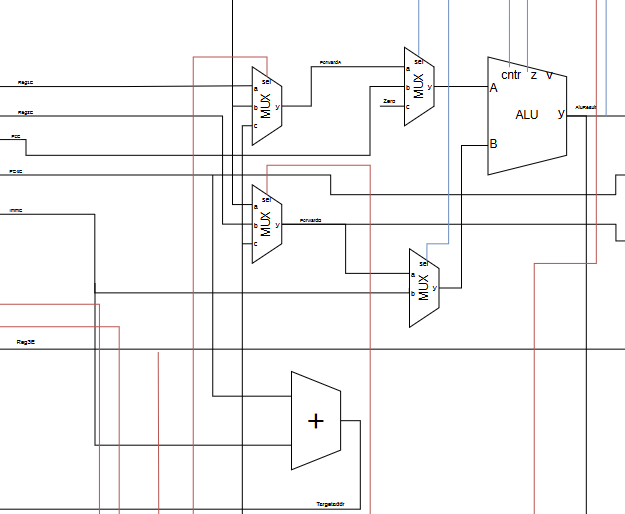
\includegraphics[scale=0.3]{Figures/Chapter 3/EX Stage.png}
	\caption{RV32ICore EX Stage}
	\label{fig:RV32ICore RV32ICore EX Stage}
\end{figure}
\section{Memory Access (MEM) Stage}
The Memory Access stage handles Load and Store instructions by interfacing with the data memory.

For Store instructions, the address computed by the ALU in the Execute stage is used as the write address, and the value of register rs2 — carried through the pipeline — is written to data memory. For Load instructions, the same computed address is used as the read address, and the data memory responds with the value stored at that location.

The data memory supports three access widths controlled by a signal derived from the Funct3 field: byte (8-bit), halfword (16-bit), and word (32-bit). For instructions that do not access memory, this stage passes the ALU result and control signals through to the Write-Back stage without interacting with the data memory.
\begin{figure}[h!]
	\centering
	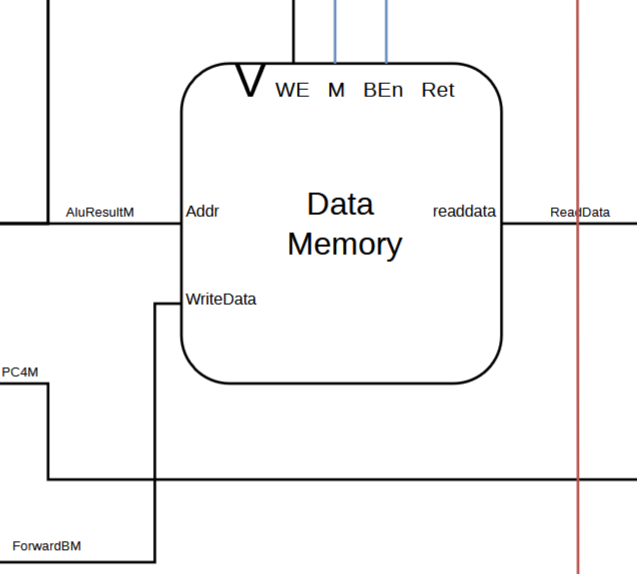
\includegraphics[scale=0.3]{Figures/Chapter 3/MEM Stage.png}
	\caption{RV32ICore MEM Stage}
	\label{fig:RV32ICore MEM Stage}
\end{figure}
\section{Write-Back (WB) Stage}
The Write-Back stage selects the value to be written to the destination register and commits it to the register file.

A Memory Extension unit first processes the raw data returned by the data memory. It performs sign extension or zero extension of byte and halfword values according to the access type specified by the Funct3 field, ensuring that the value written to the 32-bit register file conforms to the RV32I specification for load instructions.

A multiplexer then selects among three possible write-back sources: the ALU result (for arithmetic, logical, and address computation instructions), the extended memory data (for load instructions), and PC+4 (for JAL and JALR, which write the return address to the destination register). The selected value is written to the register file at the address specified by rd on the rising clock edge, completing the instruction's execution.
\begin{figure}[h!]
	\centering
	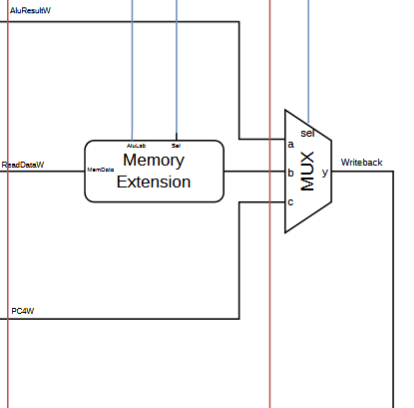
\includegraphics[scale=0.3]{Figures/Chapter 3/WR Stage.png}
	\caption{RV32ICore WR Stage}
	\label{fig:RV32ICore WR Stage}
\end{figure}
\section{Hazard Unit}
The Hazard Unit monitors the pipeline registers and intervenes when conditions arise that would cause incorrect execution. It handles three categories of hazards: data hazards, load-use hazards, and control hazards.

\subsection{Data Hazards and Forwarding}
Data hazards occur when an instruction depends on the result of a preceding instruction that has not yet been written back to the register file. RV32ICore resolves most data hazards through forwarding, which routes computed results directly from later pipeline stages back to the ALU inputs in the Execute stage, bypassing the register file.

The Hazard Unit compares the destination register of instructions in the EX/MEM and MEM/WB pipeline registers against the source registers of the instruction currently in the Execute stage. When a match is detected, forwarded values are selected at both MuxX2 and MuxX3 in place of the register file outputs. When forwarding from the MEM/WB stage following a load instruction, the forwarded value is taken from the output of the Memory Extension unit, ensuring that the correctly sign-extended loaded value is used.
\subsection{Load-Use Hazards}
A load-use hazard occurs when a load instruction is immediately followed by an instruction that uses the loaded value. Since the loaded data is not available until the end of the Memory Access stage, forwarding alone cannot resolve this hazard. The Hazard Unit detects this condition by checking whether the instruction in the Execute stage is a load and whether its destination register matches a source register of the instruction in the Decode stage. When detected, the Hazard Unit stalls the pipeline for one cycle by freezing the IF/ID and ID/EX pipeline registers and inserting a NOP into the Execute stage, allowing the loaded value to reach the MEM/WB stage where it can be forwarded.
\subsection{Control Hazards}
Control hazards arise from branch and jump instructions, whose target addresses are not known until the Execute stage. Since two instructions are fetched after every branch before its outcome is resolved, those instructions must be discarded if the branch is taken. The Hazard Unit handles this by issuing a flush signal that inserts NOP instructions into the IF/ID and ID/EX pipeline registers in the same cycle that the PC is updated to the branch target address.
\begin{figure}[h!]
	\centering
	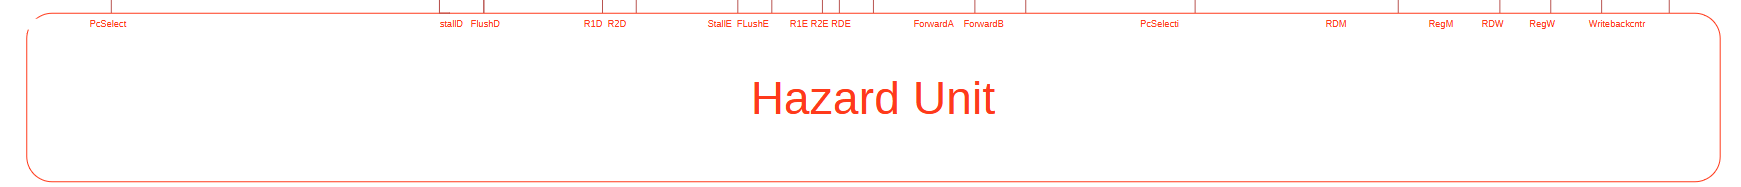
\includegraphics[scale=0.3]{Figures/Chapter 3/Hazard Unit.png}
	\caption{RV32ICore Hazard Unit}
	\label{fig:RV32ICore Hazard Unit}
\end{figure}
\section{Conclusion}
This chapter has presented the complete architecture of RV32ICore, covering its top-level decomposition into Datapath, Control Unit, and Hazard Unit, and providing a detailed description of each pipeline stage and the registers connecting them. The five-stage Harvard pipeline provides a structured and efficient framework for RV32I instruction execution. The forwarding and stalling mechanisms implemented in the Hazard Unit ensure correct execution in the presence of data dependencies, while pipeline flushing resolves control hazards introduced by branch and jump instructions. The architectural decisions described in this chapter form the direct basis for the VHDL implementation presented in the following chapter.



\chapter{Implementation \& Verification}
\section{Introduction}
This chapter presents the architecture and design of RV32ICore, a pipelined 32-bit RISC-V processor implementing the RV32I Base Integer ISA. The chapter begins with a top-level overview of the processor's major units, followed by a detailed description of each pipeline stage, the pipeline registers connecting them, and the hazard unit responsible for maintaining correct execution in the presence of data and control hazards.

\section{Top-Level Architecture}
At the highest level of abstraction, RV32ICore is composed of two primary units: the Datapath and the Control Unit, along with a dedicated Hazard Unit that operates across pipeline stages.

\textbf{The Datapath} is responsible for processing and routing data throughout the processor. Its inputs include control signals generated by the Control Unit, instructions fetched from instruction memory, and data read from data memory. Its outputs include the Program Counter (PC) supplied to instruction memory, data written to data memory, and status information such as instruction fields and condition flags fed back to the Control Unit.

\textbf{The Control Unit} is responsible for managing the correct execution of instructions by interpreting instruction fields and generating the appropriate control signals for each pipeline stage. Its inputs are the opcode (bits [6:0]), Funct3 (bits [14:12]), and Funct7 bit 30, along with the processor clock and reset. Its outputs are the set of control signals that govern the behavior of multiplexers, the register file, the ALU, and the data memory throughout the datapath.

\textbf{The Hazard Unit} monitors the pipeline state and intervenes when hazard conditions are detected. It generates stall and flush signals to preserve correct program execution in the presence of data dependencies and control flow changes. Its operation is described in detail in Section 3.9.
\begin{figure}[h!]
    \centering
    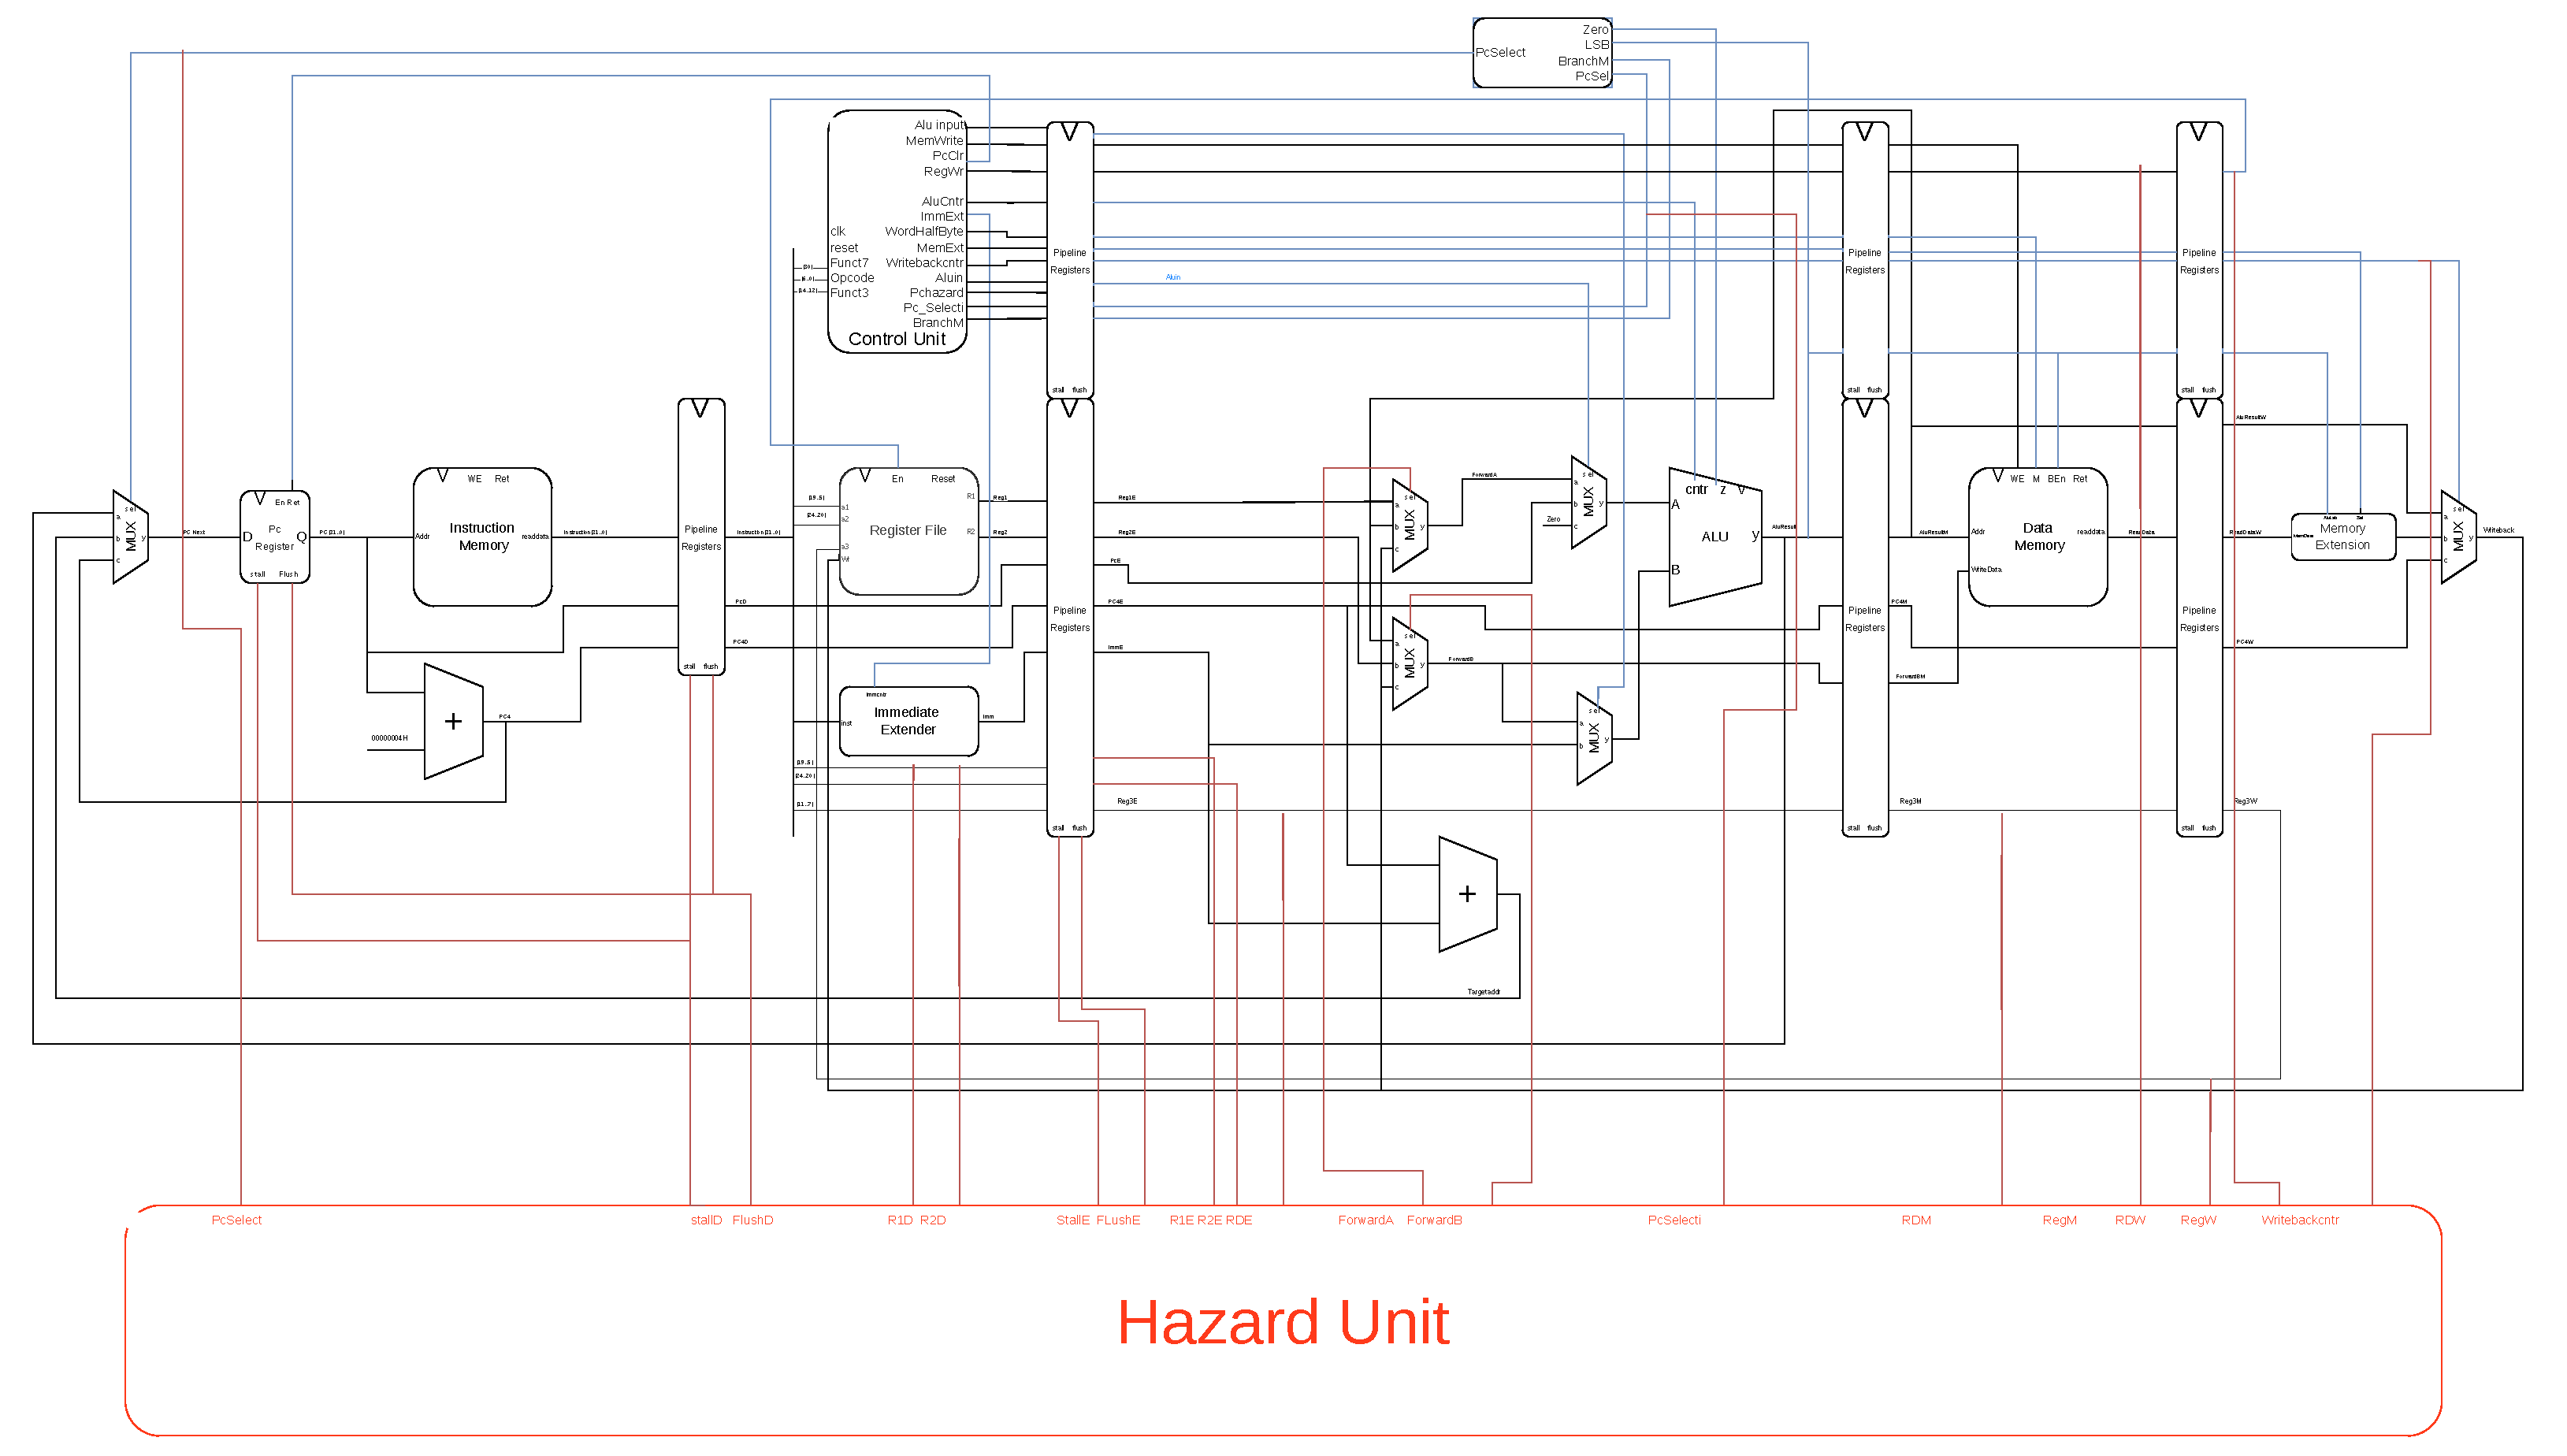
\includegraphics[scale=0.3]{Figures/Chapter 3/Top Level.pdf}
    \caption{RV32ICore Top-Level Architecture}
    \label{fig: RV32ICore Top-Level Architecture}
\end{figure}
\section{Pipeline Overview}
RV32ICore implements a classical five-stage pipeline. Pipelining allows multiple instructions to be in different stages of execution simultaneously, improving throughput by overlapping work across stages. The five stages are:

\begin{itemize}
    \item \textbf{IF} — Instruction Fetch
    \item \textbf{ID} — Instruction Decode
    \item \textbf{EX} — Execute
    \item \textbf{MEM} — Memory Access
    \item \textbf{WB} — Write-Back
\end{itemize}

Each stage is separated from the next by a pipeline register that captures the outputs of the current stage and holds them stable for the following stage on the next clock edge. All pipeline registers share the same clock as the rest of the processor and are controlled by two signals: a synchronous reset that clears the register to zero, and a NOP insertion signal that loads a harmless no-operation instruction into the register without clearing its other fields, used during flush operations.
\section{Instruction Fetch (IF) Stage}
The Instruction Fetch stage is responsible for retrieving the current instruction from instruction memory and advancing the Program Counter

The PC is stored in a dedicated register that updates on every rising clock edge under normal operation. Its value is used directly as the address supplied to the instruction memory, which responds combinationally with the 32-bit instruction word stored at that address.

A dedicated adder computes PC+4, representing the address of the next sequential instruction. This value is carried forward through the pipeline and is used in the Write-Back stage as the return address for jump instructions.

On a taken branch, the PC is updated to the branch target address computed in the Execute stage in the same cycle that the flush signal is issued. Under normal sequential execution, the PC is updated to PC+4.

The instruction memory is separate from the data memory, consistent with the Harvard architecture adopted by RV32ICore. This ensures that instruction fetch never contends with data memory access, eliminating structural hazards between the IF and MEM stages.
\begin{figure}[h!]
    \centering
    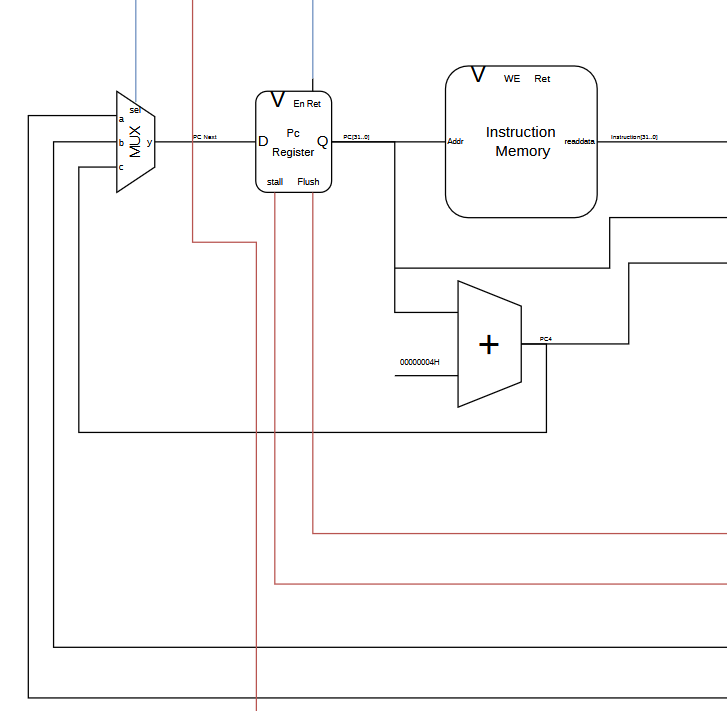
\includegraphics[scale=0.3]{Figures/Chapter 3/IF Stage.png}
    \caption{RV32ICore IF Stage}
    \label{fig: RV32ICore IF Stage}
\end{figure}
\section{Instruction Decode (ID) Stage}
The Instruction Decode stage deconstructs the fetched instruction and prepares the operands and control signals required for execution.

The 32-bit instruction word is partitioned into its constituent fields according to the RV32I specification. The source register addresses rs1 and rs2 are located at bits [19:15] and [24:20] respectively, and the destination register address rd is located at bits [11:7]. These addresses are wired directly to the read ports of the register file, which responds combinationally with the contents of the addressed registers. Register x0 is hardwired to zero; any read of x0 returns zero and any write to x0 is silently discarded.

An Immediate Extension unit receives the full 32-bit instruction word and produces a 32-bit sign-extended immediate value. The extension logic selects the appropriate immediate format — I, S, B, U, or J — based on the opcode, and assembles the immediate from the relevant instruction bits according to the RV32I encoding specification.

The opcode (bits [6:0]), Funct3 (bits [14:12]), and Funct7 bit 30 are forwarded to the Control Unit, which decodes them and generates the full set of control signals for the instruction. These control signals are stored in the ID/EX pipeline register alongside the register data and immediate value and propagate through the pipeline with the instruction.
\begin{figure}[h!]
    \centering
    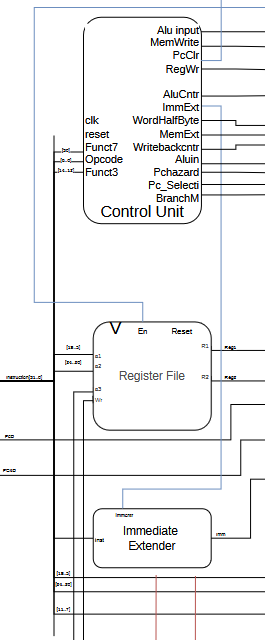
\includegraphics[scale=0.3]{Figures/Chapter 3/ID Stage.png}
    \caption{RV32ICore ID Stage}
    \label{fig: RV32ICore ID Stage}
\end{figure}
\section{Execute (EX) Stage}
The Execute stage performs the arithmetic, logical, or address computation required by the current instruction. It is the most complex stage of the datapath, containing the ALU, two input multiplexers, a branch adder, and the forwarding multiplexer logic.
\subsection{ALU Input Selection}
Two multiplexers select the operands presented to the ALU inputs.

\textbf{MuxX3} selects ALU input A from three possible sources: the value of register rs1, the current PC (used by AUIPC), or zero (used by LUI, which adds the upper immediate to zero so that the ALU result path is reused without requiring dedicated hardware). The selection is governed by a control signal generated by the Control Unit.

\textbf{MuxX2} selects ALU input B from two possible sources: the value of register rs2 (for register-to-register instructions) or the sign-extended immediate (for immediate-type instructions). The selection is governed by a corresponding control signal.

\subsection{ALU Operation}
The ALU receives the two selected operands and performs the operation specified by the ALU control signal, which is derived from the opcode, Funct3, and Funct7 fields decoded in the Control Unit. Supported operations include addition, subtraction, bitwise AND, OR, and XOR, logical and arithmetic shift, and signed and unsigned comparison. The ALU produces a 32-bit result and a zero flag used for branch condition evaluation.
\subsection{Branch Address Computation}
A dedicated adder computes the branch target address by summing the PC value carried from the IF stage with the sign-extended immediate. This target address is passed to the PC register when a branch is taken.
\subsection{Branch Resolution}
Branch conditions are evaluated in the Execute stage. When a branch is taken, the Hazard Unit issues a flush signal that inserts NOP instructions into the IF/ID and ID/EX pipeline registers in the same cycle that the PC is updated to the branch target. This discards the two incorrectly fetched instructions that entered the pipeline after the branch. No branch prediction is employed; the pipeline always flushes on a taken branch.
\begin{figure}[h!]
    \centering
    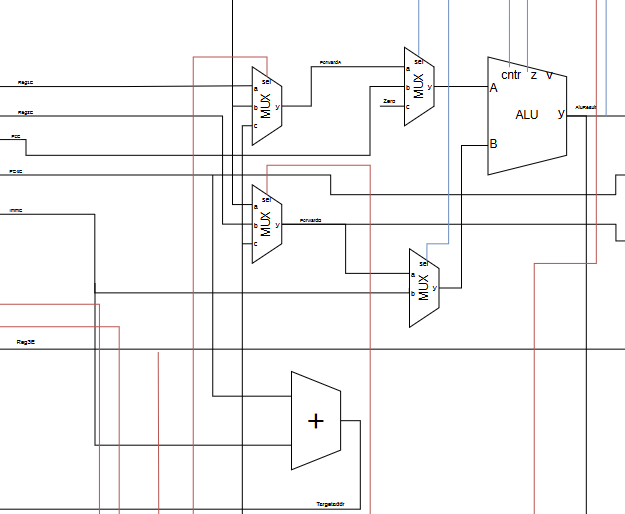
\includegraphics[scale=0.3]{Figures/Chapter 3/EX Stage.png}
    \caption{RV32ICore EX Stage}
    \label{fig:RV32ICore RV32ICore EX Stage}
\end{figure}
\section{Memory Access (MEM) Stage}
The Memory Access stage handles Load and Store instructions by interfacing with the data memory.

For Store instructions, the address computed by the ALU in the Execute stage is used as the write address, and the value of register rs2 — carried through the pipeline — is written to data memory. For Load instructions, the same computed address is used as the read address, and the data memory responds with the value stored at that location.

The data memory supports three access widths controlled by a signal derived from the Funct3 field: byte (8-bit), halfword (16-bit), and word (32-bit). For instructions that do not access memory, this stage passes the ALU result and control signals through to the Write-Back stage without interacting with the data memory.
\begin{figure}[h!]
    \centering
    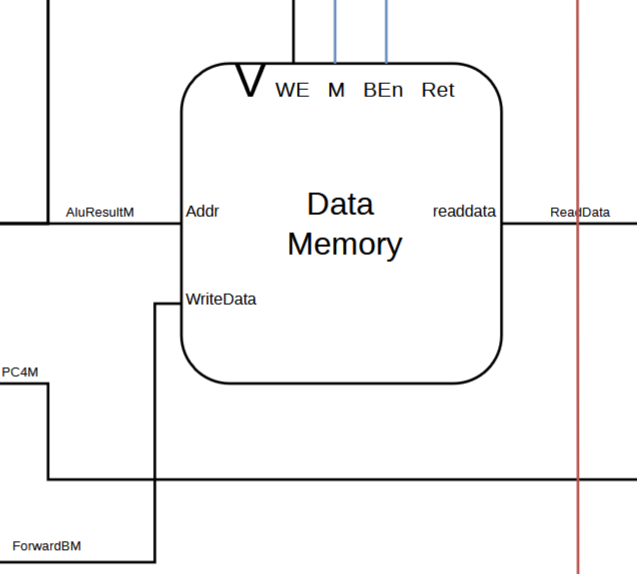
\includegraphics[scale=0.3]{Figures/Chapter 3/MEM Stage.png}
    \caption{RV32ICore MEM Stage}
    \label{fig:RV32ICore MEM Stage}
\end{figure}
\section{Write-Back (WB) Stage}
The Write-Back stage selects the value to be written to the destination register and commits it to the register file.

A Memory Extension unit first processes the raw data returned by the data memory. It performs sign extension or zero extension of byte and halfword values according to the access type specified by the Funct3 field, ensuring that the value written to the 32-bit register file conforms to the RV32I specification for load instructions.

A multiplexer then selects among three possible write-back sources: the ALU result (for arithmetic, logical, and address computation instructions), the extended memory data (for load instructions), and PC+4 (for JAL and JALR, which write the return address to the destination register). The selected value is written to the register file at the address specified by rd on the rising clock edge, completing the instruction's execution.
\begin{figure}[h!]
    \centering
    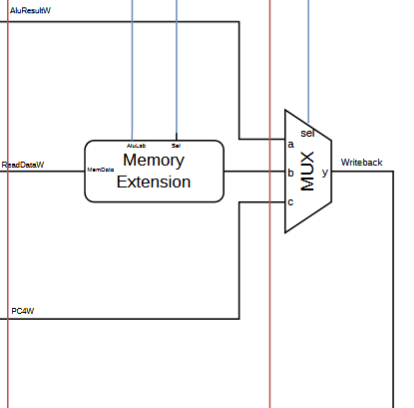
\includegraphics[scale=0.3]{Figures/Chapter 3/WR Stage.png}
    \caption{RV32ICore WR Stage}
    \label{fig:RV32ICore WR Stage}
\end{figure}
\section{Hazard Unit}
The Hazard Unit monitors the pipeline registers and intervenes when conditions arise that would cause incorrect execution. It handles three categories of hazards: data hazards, load-use hazards, and control hazards.

\subsection{Data Hazards and Forwarding}
Data hazards occur when an instruction depends on the result of a preceding instruction that has not yet been written back to the register file. RV32ICore resolves most data hazards through forwarding, which routes computed results directly from later pipeline stages back to the ALU inputs in the Execute stage, bypassing the register file.

The Hazard Unit compares the destination register of instructions in the EX/MEM and MEM/WB pipeline registers against the source registers of the instruction currently in the Execute stage. When a match is detected, forwarded values are selected at both MuxX2 and MuxX3 in place of the register file outputs. When forwarding from the MEM/WB stage following a load instruction, the forwarded value is taken from the output of the Memory Extension unit, ensuring that the correctly sign-extended loaded value is used.
\subsection{Load-Use Hazards}
A load-use hazard occurs when a load instruction is immediately followed by an instruction that uses the loaded value. Since the loaded data is not available until the end of the Memory Access stage, forwarding alone cannot resolve this hazard. The Hazard Unit detects this condition by checking whether the instruction in the Execute stage is a load and whether its destination register matches a source register of the instruction in the Decode stage. When detected, the Hazard Unit stalls the pipeline for one cycle by freezing the IF/ID and ID/EX pipeline registers and inserting a NOP into the Execute stage, allowing the loaded value to reach the MEM/WB stage where it can be forwarded.
\subsection{Control Hazards}
Control hazards arise from branch and jump instructions, whose target addresses are not known until the Execute stage. Since two instructions are fetched after every branch before its outcome is resolved, those instructions must be discarded if the branch is taken. The Hazard Unit handles this by issuing a flush signal that inserts NOP instructions into the IF/ID and ID/EX pipeline registers in the same cycle that the PC is updated to the branch target address.
\begin{figure}[h!]
    \centering
    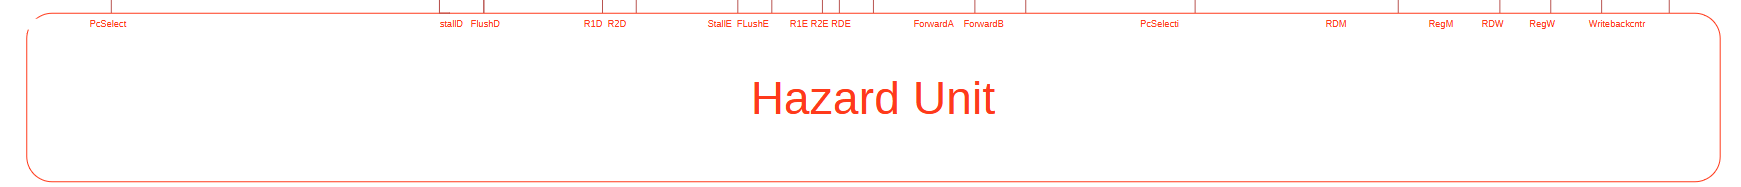
\includegraphics[scale=0.3]{Figures/Chapter 3/Hazard Unit.png}
    \caption{RV32ICore Hazard Unit}
    \label{fig:RV32ICore Hazard Unit}
\end{figure}
\section{Conclusion}
This chapter has presented the complete architecture of RV32ICore, covering its top-level decomposition into Datapath, Control Unit, and Hazard Unit, and providing a detailed description of each pipeline stage and the registers connecting them. The five-stage Harvard pipeline provides a structured and efficient framework for RV32I instruction execution. The forwarding and stalling mechanisms implemented in the Hazard Unit ensure correct execution in the presence of data dependencies, while pipeline flushing resolves control hazards introduced by branch and jump instructions. The architectural decisions described in this chapter form the direct basis for the VHDL implementation presented in the following chapter.



\chapter{IDS Theoretical Background \& System Architecture}
\section{Introduction}
This chapter describes the implementation of RV32ICore in VHDL, covering the structural organization of the design, the implementation of each major component, key design decisions made during development, and the toolchain used to compile and load test programs into the simulation environment. The implementation follows directly from the architecture described in Chapter 3, with each architectural unit realized as a distinct VHDL entity.    

\section{Design Philosophy}

The IDS is structured as a linear pipeline of independent modules, each consuming the same byte stream that flows from a physical interface receiver. Parsers at different protocol layers operate simultaneously on the same data; rule checkers fire one clock cycle after their corresponding parser completes. This means the system does not buffer a full packet before beginning inspection---field extraction and rule evaluation are interleaved with frame reception.

The choice of a byte-stream interface as the internal contract between modules makes each module independently testable and allows the physical reception mechanism to be swapped (from RMII simulation to AXI-Stream DMA for hardware) without modifying any parser or checker.

\section{Top-Level Structure}

The pipeline is wired together in a single top-level entity, \texttt{ids\_top.vhd}. It instantiates all sub-modules and connects them through internal signals. The byte stream---\texttt{rx\_byte}, \texttt{rx\_valid}, \texttt{rx\_sof}, \texttt{rx\_eof}---is broadcast to every parser simultaneously.

% --- FIGURE PLACEHOLDER ---
% Replace with the IDS pipeline diagram (Image 1 from your PNGs)
%
\begin{figure}[H]
	\centering
	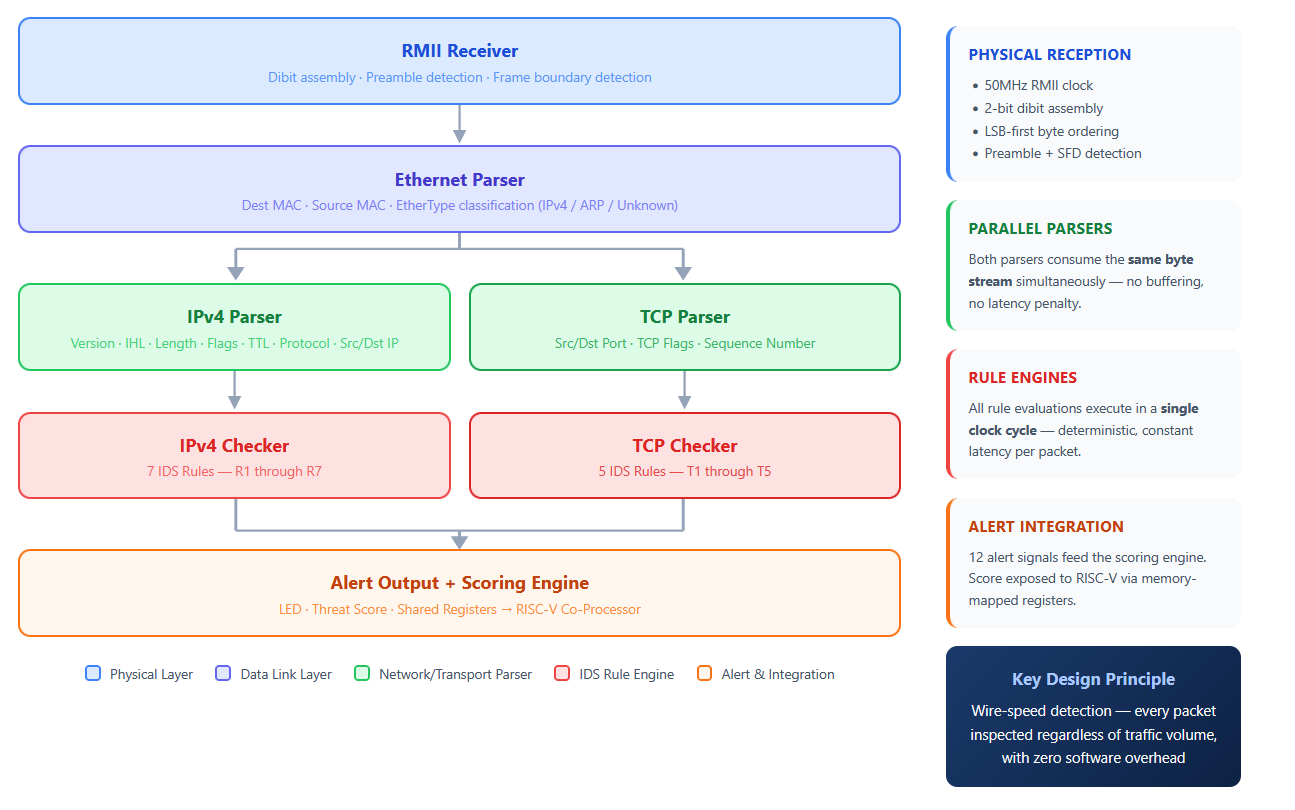
\includegraphics[width=0.95\textwidth]{ids_pipeline_diagram.png}
	\caption{IDS pipeline architecture showing parallel parsers and rule engines.}
	\label{fig:pipeline}
\end{figure}

\noindent The four-signal byte-stream interface carries the following semantics:
\begin{itemize}
	\item \texttt{rx\_sof} pulses for one clock cycle at the start of a new frame.
	\item \texttt{rx\_byte} / \texttt{rx\_valid} delivers one byte per clock when valid.
	\item \texttt{rx\_eof} pulses for one clock cycle at the end of the frame.
\end{itemize}

This interface is the internal standard across all modules.

\section{RMII Receiver (\texttt{rmii\_rx.vhd})}

In simulation, Ethernet frames are injected using RMII signalling: two data bits (a \emph{dibit}) are presented every clock cycle at 50\,MHz, LSB-first. The RMII receiver is a three-state FSM (IDLE, PREAMBLE, DATA) that assembles four consecutive dibits into one byte using a right-shift register:

\begin{lstlisting}[caption={Dibit assembly in \texttt{rmii\_rx.vhd}}, label=lst:rmii]
	shift_reg <= rmii_rxd & shift_reg(7 downto 2);
	if dibit_cnt = "11" then
	rx_byte  <= rmii_rxd & shift_reg(7 downto 2);
	rx_valid <= '1';
	end if;
\end{lstlisting}

The preamble state counts at least eight \texttt{01} dibits before accepting the Start Frame Delimiter (\texttt{11}). On hardware, this module is replaced by an AXI-Stream receiver that accepts bytes directly from the PS DMA engine; the rest of the pipeline is unchanged.

\section{Ethernet Parser (\texttt{eth\_parser.vhd})}

The Ethernet parser extracts the destination MAC, source MAC, and EtherType from the first 14 bytes of each frame. It uses a sequential FSM with states for each header field group (DST\_MAC, SRC\_MAC, ETHERTYPE, PAYLOAD, DONE). On the DONE state, it asserts \texttt{frame\_done} and one of \texttt{is\_ipv4}, \texttt{is\_arp}, or \texttt{is\_unknown} based on the EtherType value (0x0800, 0x0806, or other).

A key design decision is that all output signals default to \texttt{'0'} at the top of the clocked process and are only overridden in the DONE state. This prevents latches and ensures outputs are valid for exactly one clock cycle.

\section{Frame Counter (\texttt{frame\_counter.vhd})}

The frame counter accumulates per-second frame statistics (total, IPv4, ARP, unknown) using a hardware divider: a counter incremented every clock cycle triggers a \texttt{one\_sec\_tick} when it reaches \texttt{CLK\_FREQ\_HZ - 1}. On that tick, the running accumulators are latched to output registers and reset. This value is passed as a generic so the same code simulates at \texttt{CLK\_FREQ\_HZ = 1000} (1\,kHz) and synthesizes at \texttt{CLK\_FREQ\_HZ = 50\,000\,000} (50\,MHz), making testbenches fast without any code changes.

\section{IPv4 Parser (\texttt{ipv4\_parser.vhd})}

The IPv4 parser skips the 14-byte Ethernet header (counted in the ETH\_HEADER state) and then extracts the following fields from the IP header:

\begin{table}[H]
	\centering
	\caption{IPv4 header fields extracted by \texttt{ipv4\_parser.vhd}}
	\label{tab:ipv4fields}
	\begin{tabular}{lll}
		\toprule
		\textbf{Field} & \textbf{Byte offset} & \textbf{Width} \\
		\midrule
		Version / IHL   & 0      & 4 + 4 bits \\
		Total Length    & 2--3   & 16 bits    \\
		Flags / Fragment Offset & 6--7 & 3 + 13 bits \\
		TTL             & 8      & 8 bits     \\
		Protocol        & 9      & 8 bits     \\
		Source IP       & 12--15 & 32 bits    \\
		Destination IP  & 16--19 & 32 bits    \\
		\bottomrule
	\end{tabular}
\end{table}

The IHL field determines where the IP header ends (IHL\,$\times$\,4 bytes). The parser computes this boundary dynamically and transitions to WAIT\_EOF once all header bytes have been consumed, asserting \texttt{parse\_done} and \texttt{parse\_valid} (the latter only when \texttt{ip\_version = 4}) after the frame ends.

\section{IPv4 Checker (\texttt{ipv4\_checker.vhd})}

The IPv4 checker receives the parsed fields when \texttt{parse\_done} is asserted and evaluates all rules combinatorially inside a clocked process in a single clock cycle. A local variable \texttt{any\_alert} is OR'd across all rule conditions and drives the \texttt{alert\_any} output. Individual alert signals (\texttt{alert\_bad\_version}, \texttt{alert\_fragment}, etc.) are also driven, allowing the scoring engine to weight them differently.

\section{TCP Parser (\texttt{tcp\_parser.vhd})}

The TCP parser shares the same byte stream as the IPv4 parser. Because the TCP header begins at a byte offset that depends on the IP IHL field, the parser captures \texttt{ip\_ihl} and \texttt{ip\_protocol} from the IPv4 parser's output signals before the frame starts. It then skips to byte \texttt{14 + IHL\,$\times$\,4} (Ethernet header + IP header) before beginning TCP field extraction.

Fields extracted: source port, destination port, sequence number, and the flags byte. The flags byte at offset 13 of the TCP header encodes FIN, SYN, RST, PSH, ACK, and URG in bits 0--5.

\section{TCP Checker (\texttt{tcp\_checker.vhd})}

The TCP checker uses VHDL \texttt{alias} declarations to give readable names to individual flag bits:

\begin{lstlisting}[caption={Flag aliases in \texttt{tcp\_checker.vhd}}, label=lst:aliases]
	alias flag_fin : std_logic is tcp_flags(0);
	alias flag_syn : std_logic is tcp_flags(1);
	alias flag_rst : std_logic is tcp_flags(2);
\end{lstlisting}

Rules are expressed directly as Boolean conditions on these aliases, making the intent clear without bit-masking arithmetic.

\section{UDP Parser (\texttt{udp\_parser.vhd})}

The UDP header is 8 bytes long: source port (2), destination port (2), length (2), and checksum (2). The parser reuses the same skip-to-transport-layer logic as the TCP parser, activated only when \texttt{ip\_protocol = 0x11}. The \texttt{parse\_valid} output is asserted only for UDP packets.

\section{UDP Checker (\texttt{udp\_checker.vhd})}

The UDP checker evaluates nine rules on the extracted UDP fields and a configurable set of forbidden port values, shared with the TCP checker through the rule register bank.

% ============================================================
\section{Detection Rules}
\label{ch:rules}
% ============================================================

\subsection{Overview}

The IDS evaluates twenty detection rules across four protocol layers. Rules are grouped by the checker module that evaluates them. Each rule fires for exactly one clock cycle when its condition is met; the alert is latched and its weight added to the threat score.

\subsection{IPv4 Rules (R1--R12)}

\subsubsection{Rules R1--R7: Core Validity Checks}

These seven rules detect structurally malformed or trivially suspicious IPv4 packets.

\begin{table}[H]
	\centering
	\caption{IPv4 detection rules R1--R7}
	\label{tab:r1r7}
	\begin{tabular}{lll}
		\toprule
		\textbf{Rule} & \textbf{Condition} & \textbf{Attack / Anomaly} \\
		\midrule
		R1 & \texttt{ip\_version} $\neq$ 4          & Non-IPv4 / malformed packet \\
		R2 & \texttt{ip\_ihl} $<$ 5                  & Invalid header length       \\
		R3 & \texttt{ip\_length} $<$ 20              & Impossible packet size      \\
		R4 & \texttt{ip\_ttl} $\leq$ 1              & Suspicious TTL / traceroute \\
		R5 & \texttt{ip\_frag\_off} $>$ 0           & Fragmentation attack        \\
		R6 & \texttt{ip\_src} = \texttt{0.0.0.0}   & Spoofed source address      \\
		R7 & \texttt{ip\_src} = \texttt{ip\_dst}   & Land attack                 \\
		\bottomrule
	\end{tabular}
\end{table}

\subsubsection{Rules R8--R12: Bogon and Header Abuse}

These five rules detect packets whose source addresses belong to reserved or unroutable address blocks, or whose header fields abuse optional mechanisms.

\begin{table}[H]
	\centering
	\caption{IPv4 detection rules R8--R12}
	\label{tab:r8r12}
	\begin{tabular}{lll}
		\toprule
		\textbf{Rule} & \textbf{Condition} & \textbf{Attack / Anomaly} \\
		\midrule
		R8  & \texttt{ip\_src[31:24]} = \texttt{0x7F}          & Loopback source (127.x.x.x)        \\
		R9  & \texttt{ip\_src[31:16]} = \texttt{0xA9FE}        & Link-local source (169.254.x.x)    \\
		R10 & \texttt{ip\_src[31:28]} = \texttt{0xE}           & Multicast source (224--239.x.x.x) \\
		R11 & \texttt{ip\_ihl} $>$ 5                           & IP options present                  \\
		R12 & \texttt{ip\_flags[2]} = \texttt{'1'}             & Reserved IPv4 flag bit set          \\
		\bottomrule
	\end{tabular}
\end{table}

Rules R8--R10 share a single enable bit (\texttt{bogon\_check\_en}) in the rule register bank so the RISC-V can disable them all at once on a network segment where such addresses may legitimately appear.

\subsection{TCP Rules (T1--T5)}

\begin{table}[H]
	\centering
	\caption{TCP detection rules T1--T5}
	\label{tab:t1t5}
	\begin{tabular}{lll}
		\toprule
		\textbf{Rule} & \textbf{Condition} & \textbf{Attack / Anomaly} \\
		\midrule
		T1 & SYN = 1 and FIN = 1                    & Illegal flag combination    \\
		T2 & SYN = 1 and RST = 1                    & Illegal flag combination    \\
		T3 & All flags = \texttt{0x00}              & NULL scan (port probe)      \\
		T4 & All flags = \texttt{0xFF}              & XMAS scan (port probe)      \\
		T5 & \texttt{dst\_port} $\in$ forbidden set & Access to forbidden service \\
		\bottomrule
	\end{tabular}
\end{table}

The forbidden port set (rule T5) is stored in configurable registers and defaults to Telnet (23), FTP (21), and TFTP (69). The RISC-V processor can update these values without reprogramming the FPGA.

\subsection{UDP Rules (U1--U9)}

\begin{table}[H]
	\centering
	\caption{UDP detection rules U1--U9}
	\label{tab:u1u9}
	\begin{tabular}{lp{6cm}p{6cm}}
		\toprule
		\textbf{Rule} & \textbf{Condition} & \textbf{Attack / Anomaly} \\
		\midrule
		U1 & \texttt{udp\_dst\_port} $\in$ forbidden set & Access to forbidden UDP service \\
		U2 & \texttt{udp\_length} $<$ 8 & Invalid UDP length field \\
		U3 & \texttt{udp\_length} $=$ 0 & Completely malformed UDP packet \\
		U4 & \texttt{udp\_src\_port} $\in$ \{53, 123, 11211, 19\} & Amplification attack response (DNS/NTP/Memcached/CHARGEN) \\
		U5 & \texttt{ip\_src} $=$ \texttt{ip\_dst} $\wedge$ \texttt{udp\_src\_port} $=$ \texttt{udp\_dst\_port} & UDP land attack \\
		U6 & \texttt{udp\_length} $>$ 1472 & Oversized datagram (exceeds Ethernet MTU) \\
		U7 & \texttt{udp\_src\_port} $=$ 0 $\vee$ \texttt{udp\_dst\_port} $=$ 0 & Reserved port zero used \\
		U8 & \texttt{udp\_dst\_port} $=$ 1900 & SSDP/UPnP abuse \\
		U9 & \texttt{udp\_dst\_port} $=$ 11211 & Memcached amplification request \\
		\bottomrule
	\end{tabular}
\end{table}
\newpage
\subsection{Alert Weighting}

Each alert type is assigned a weight, and the scoring engine accumulates weights additively. The RISC-V classifies traffic into three severity tiers based on the accumulated score.
\begin{table}[H]
	\centering
	\caption{Alert weights used by the scoring engine}
	\label{tab:weights}
	\begin{tabular}{llr}
		\toprule
		\textbf{Alert} & \textbf{Rule} & \textbf{Weight} \\
		\midrule
		Bad version          & R1       & 5  \\
		Bad IHL              & R2       & 5  \\
		Bad length           & R3       & 10 \\
		Low TTL              & R4       & 5  \\
		Fragmentation        & R5       & 15 \\
		Spoofed source       & R6       & 20 \\
		Land attack          & R7       & 25 \\
		Bogon source         & R8--R10  & 15 \\
		IP options           & R11      & 10 \\
		Reserved flag        & R12      & 10 \\
		SYN+FIN              & T1       & 25 \\
		SYN+RST              & T2       & 20 \\
		NULL scan            & T3       & 20 \\
		XMAS scan            & T4       & 20 \\
		Forbidden TCP port   & T5       & 15 \\
		Forbidden UDP port   & U1       & 15 \\
		Malformed UDP length & U2, U3   & 10 \\
		Amplification resp.  & U4       & 20 \\
		UDP land attack      & U5       & 25 \\
		Oversized UDP        & U6       & 10 \\
		Port zero            & U7       & 10 \\
		SSDP/UPnP abuse      & U8       & 15 \\
		Memcached amplif.    & U9       & 20 \\
		\bottomrule
	\end{tabular}
\end{table}

The score decays by a configurable rate every second when no new alerts fire, preventing a historical event from permanently elevating the severity level.



\chapter{Implementation \& Testing}
\section{Introduction}
\paragraph{}
A processor is considered functionally correct when it successfully executes the complete set of target ISA instructions, producing results consistent with the architectural specification. To verify RV32ICore, a set of C programs of increasing complexity are compiled using the xPack RISC-V GCC toolchain and executed in simulation. Correct execution is determined by inspecting the values held in memory or the register file at the end of simulation and comparing them against analytically computed expected results. 
\section{Simulation Environment:}
Most of the tests performed on RV32ICore will follow a structured simulation environment. The environment contains:
\subsection{Testbench Code:}
\begin{minted}[baselinestretch=1]{vhdl}
	Library ieee;
	use ieee.std_logic_1164.all;
	entity Hazard_Testbench is
	end entity;
	
	architecture arch of Hazard_Testbench is
	component P_Processor_Hazard is
	port(...
	);
	end component;
	component RAM_Inst is
	port(...
	);
	end component;
	component RAM is
	port(...
	);
	end component;
	Signal clk ,reset: std_logic;
	Signal instruction, ReadData: std_logic_vector(31 downto 0);
	Signal MemWrite: std_logic;
	Signal ByteEn, Mode: std_logic_vector(1 downto 0);
	Signal Pc: std_logic_vector(31 downto 0);
	Signal DataAdr, WriteData: std_logic_vector(31 downto 0);
	Signal clk_cnt, Inst_Change_Cnt: integer := 0;--number Of clocks counter
	begin
	UUT: P_Processor_Hazard port map(...
	);
	Data_RAM: RAM port map(...
	);
	Inst_RAM: RAM_Inst port map(...
	);
	clock: process Begin
	loop
	clk<= '1';
	wait for 10 ns;
	clk<= '0';
	wait for 10 ns;
	end loop;
	end process;
	
	Clock_counter: process(clk) 
	variable last: std_logic_vector(31 downto 0);
	Begin
	if(rising_edge(clk)) then
	clk_cnt<= clk_cnt + 1;
	if (instruction /= last) then
	Inst_Change_Cnt <= Inst_Change_Cnt + 1;
	end if;
	last := instruction;
	end if;
	end process;
	
	Stimulus: process Begin
	reset<= '1';
	wait for 40 ns;
	reset<= '0';
	wait;
	end process;
	end architecture;
\end{minted}
\label{RV32ICore Testbench Code}
The code maps between the processor and its memories and defines the necessary signals to do so. The testbench initializes by applying a reset for two clock cycles ensuring that the Pc, register file, and memory are all starting with Zero. A clock of 20 ns period is simulated using a Clock process and wait commands, and a counter is added to calculate the number of instructions preformed in a program used to calculate performance.
\subsection{Memory Loading}
The programs used for testing can be very long making impractical to load them manually. A more efficient way is to use the compiler. The output file can be turned into an output hex file which can be directly loaded into memory using a command supported by ModelSim (mem load -infile output.hex -format hex \allowbreak  sim:/hazard\_testbench/Inst\_RAM/Mem\allowbreak).
\subsection{Running The Simulation}
By running the simulation for an appropriate amount of time the results generated by the processor can be verified in memory where they are stored. Additionally if a it is necessary to check the behavior of any signal during the processing it is possible to do so using Waveforms.
\section{Tests}
Two tests will be preformed one of a summing function called by main and the other is more complex containing multiple arithmetic functions.
\subsection{Test N:°1}

The Processor initialize by resetting for two clock periods the PC starts with address 0 and increment by 4 in Normal sequence (No execution flow instructions) instructions are being fetched as the waveform suggests.

\pagebreak

\begin{figure}[h!]
	\centering
	
\includegraphics[width=0.7\linewidth]{C:/Users/dell/Pictures/Screenshots/Waveform}
	\caption{R32ICore Initialization}
	\label{fig:waveform}
\end{figure}

When the execution of the program ends we can check the final values stored in stack due to instruction
\begin{minted}{riscv}
	E4:	sw  a0,-20(s0) ; [000003BC] = a0 where a0= 16H
\end{minted}
The following Figure indicates that indeed the program executed as expected by computing the value 16H and storing it in location address 0x000003BC, which when divided by the word size of 4 bytes corresponds to word index 0xEF in the data memory.
\begin{figure}[h!]
	\centering
	\includegraphics[width=0.7\linewidth]{"C:/Users/dell/Pictures/Screenshots/Sum array result"}
	\caption{Sum Array Result}
	\label{fig:sum-array-result}
\end{figure}
With this result it is appropriate to say that the processor is working properly another test will be done for further verification.
\subsection{Test N:°2}
The second test uses the following C code. It contains the previously used array summer it also contains a multiplayer, a pointer manipulator, and a bit-wise manipulator. The analyzed values should be 16H, 78H, 09H, and 08H respectively. 
\begin{minted}[baselinestretch=1]{c}
	// test.c
	
	// Tests loops and addition
	int sum_array(int arr[], int len) {
		int sum = 0;
		for (int i = 0; i < len; i++) {
			sum += arr[i];
		}
		return sum;
	}
	
	// Tests recursion and stack depth
	int factorial(int n) {
		int result = 1; // multiply by repeated addition
		for (int i = 2; i <= n; i++) {
			int temp = 0;
			for (int j = 0; j < i; j++) {
				temp += result;  
			}
			result = temp;
		}
		return result;
	}
	// Tests pointer manipulation
	int find_max(int arr[], int len) {
		int max = arr[0];
		for (int i = 1; i < len; i++) {
			if (arr[i] > max)
			max = arr[i];
		}
		return max;
	}
	
	// Tests bitwise operations
	unsigned int count_bits(unsigned int n) {
		unsigned int count = 0;
		while (n) {
			count += n & 1;
			n >>= 1;
		}
		return count;
	}
	
	int main() {
		int arr[] = {3, 7, 2, 9, 1};
		int s = sum_array(arr, 5);       // expected: 22
		int f = factorial(5);             // expected: 120
		int m = find_max(arr, 5);        // expected: 9
		unsigned int b = count_bits(255); // expected: 8
		return 0;
	}
\end{minted}
By checking the contents of the memory we find.
\begin{figure}[h!]
	\centering
	\includegraphics[width=0.7\linewidth]{"C:/Users/dell/Pictures/Screenshots/Second Test"}
	\caption{Second Test Results}
	\label{fig:second-test}
\end{figure}

The processor is preforming as intended and further testing was done on the unused instructions by the previous programs. 
\section{Conclusion}
\paragraph{}
This chapter has presented the verification methodology and simulation results for RV32ICore. A structured testing approach was adopted in which C programs of increasing complexity were compiled using the xPack RISC-V GCC toolchain and executed in the ModelSim simulation environment. 
\paragraph{}
Correct execution was determined by comparing values stored in the data memory against analytically derived expected results, with complete assembly listings provided in the Appendix for reference. Reset behavior was verified to be correct, with the PC initializing to zero and the pipeline filling in proper sequence following reset release. Two principal test programs were used: the first verified loop execution, load and store operations, and basic arithmetic through a sum-of-array computation producing the correct result of 22 (0x16); the second subjected the processor to a more demanding workload involving multiple concurrent function calls, factorial computation, pointer manipulation, and bitwise operations, yielding the correct results of 22, 120, 9, and 8 respectively. The remaining RV32I instructions were individually verified through targeted test programs. The combined results confirm that RV32ICore correctly executes the full RV32I Base Integer ISA under simulation.


\chapter{System Integration}
\section{Hardware Platform}
The MicroPhase Z7-Lite combines an ARM Cortex-A9 PS and Artix-7-equivalent PL in a single Zynq-7020 SoC. The on-board RTL8201F Ethernet PHY connects to the PS via RGMII, so the MAC and PHY interface are handled entirely within the PS. The PL cannot directly observe raw Ethernet traffic; raw packet bytes must be passed from PS to PL.

\begin{table}[H]
	\centering
	\caption{Z7-Lite PL pin assignments}
	\begin{tabular}{lll}
		\toprule
		\textbf{Signal} & \textbf{Pin} & \textbf{Function} \\
		\midrule
		\texttt{PL\_CLK\_50M} & N18 & 50\,MHz main clock \\
		\texttt{PL\_LED1}     & P15 & \texttt{led\_alert} output \\
		\texttt{GPIO1\_17N}   & U12 & \texttt{led\_active} output \\
		\texttt{PL\_KEY1}     & P16 & Active-low reset \\
		\bottomrule
	\end{tabular}
	\label{tab:pins}
\end{table}

\section{PS-to-PL Packet Forwarding}
The PS ARM receives complete Ethernet frames via the GigE MAC, strips the 4-byte FCS, and writes the frame into a DMA buffer. The AXI-Stream DMA IP transfers the buffer to PL fabric, where \texttt{axis\_rx.vhd} converts AXI-Stream signals (\texttt{tvalid}, \texttt{tready}, \texttt{tdata}, \texttt{tlast}) into the internal byte-stream interface. The entire parser and checker stack is unchanged for hardware use.

\begin{figure}[H]
	\centering
	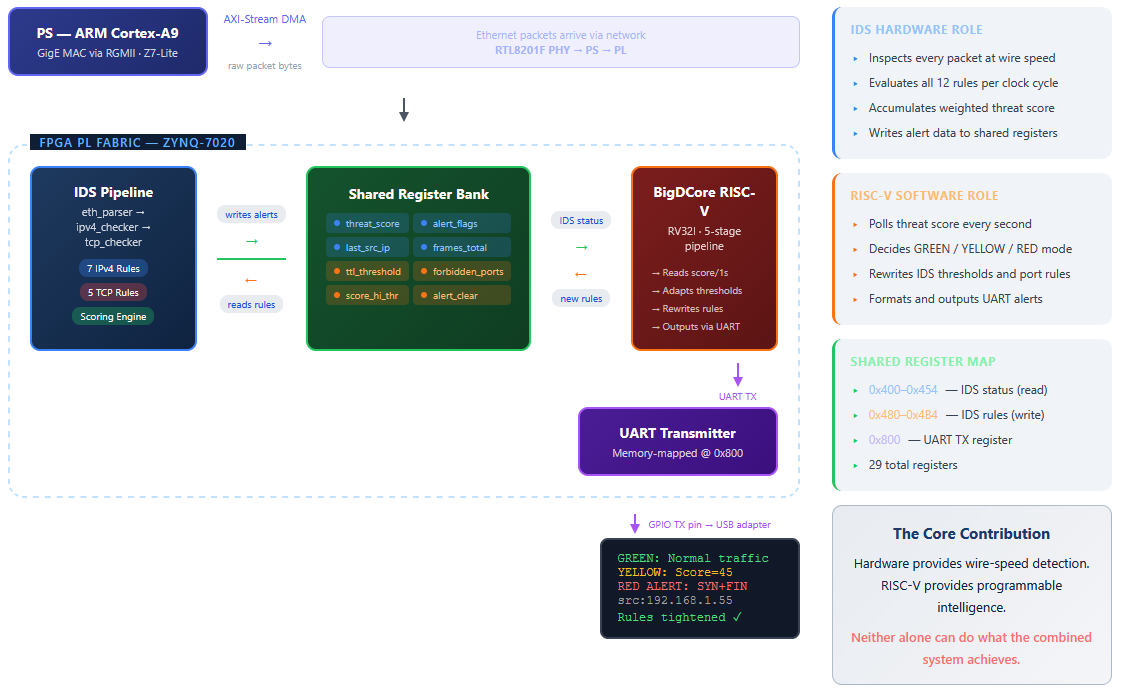
\includegraphics[width=0.95\textwidth]{integration_diagram.png}
	\caption{PS-PL co-design: packet path from RTL8201F through AXI-Stream DMA to the IDS pipeline, with shared register bank connecting IDS to RV32ICore.}
	\label{fig:integration}
\end{figure}

The \texttt{axis\_rx.vhd} wrapper asserts \texttt{tready} permanently and maps: \texttt{tvalid}$\to$\texttt{rx\_valid}, \texttt{tdata[7:0]}$\to$\texttt{rx\_byte}, \texttt{tlast}$\to$\texttt{rx\_eof}, and a one-cycle delayed \texttt{tvalid} rising edge$\to$\texttt{rx\_sof}.

\section{RISC-V Co-Processor Integration}

\subsection{Shared Register Bank}
RV32ICore exposes a standard external memory interface (\texttt{DataAdr}, \texttt{ReadData}, \texttt{WriteData}, \texttt{MemWrite}, \texttt{ByteEn}, \texttt{Mode}), so IDS registers appear to the processor as ordinary memory locations. The shared register bank (\texttt{shared\_regs.vhd}) implements 29 32-bit registers at addresses \texttt{0x400--0x4B4}:

\begin{itemize}
	\item \textbf{Status registers (0x400--0x454)} — written by IDS, read by RISC-V: threat score, 12-bit alert flags bitmask, cumulative alert counts, per-protocol frame counts, frames-per-second statistics, and last-alerted packet fields.
	\item \textbf{Rule registers (0x480--0x4B4)} — written by RISC-V, read by IDS: TTL threshold, fragmentation check enable, scoring thresholds, score decay rate, alert clear command, and eight configurable forbidden port values.
\end{itemize}

\begin{table}[H]
	\centering
	\caption{Shared register map (selected entries)}
	\begin{tabular}{lll}
		\toprule
		\textbf{Address} & \textbf{Register} & \textbf{Direction} \\
		\midrule
		0x400 & \texttt{threat\_score}          & IDS $\rightarrow$ RISC-V \\
		0x404 & \texttt{alert\_flags}           & IDS $\rightarrow$ RISC-V \\
		0x428 & \texttt{fps\_total}             & IDS $\rightarrow$ RISC-V \\
		0x434 & \texttt{last\_alert\_src\_ip}   & IDS $\rightarrow$ RISC-V \\
		0x454 & \texttt{threat\_level}          & IDS $\rightarrow$ RISC-V \\
		0x480 & \texttt{ttl\_threshold}         & RISC-V $\rightarrow$ IDS \\
		0x490 & \texttt{score\_decay\_rate}     & RISC-V $\rightarrow$ IDS \\
		0x494 & \texttt{alert\_clear}           & RISC-V $\rightarrow$ IDS \\
		0x498 & \texttt{forbidden\_port\_0}     & RISC-V $\rightarrow$ IDS \\
		0x800 & \texttt{uart\_tx}               & RISC-V $\rightarrow$ UART \\
		\bottomrule
	\end{tabular}
	\label{tab:regmap}
\end{table}

\subsection{Adaptive Threat Scoring}
The threat score accumulates alert weights each clock cycle and decays by a configurable rate every second. The RISC-V polls the score register at one-second intervals and maps it to three severity levels:

\begin{itemize}
	\item \textbf{GREEN} (score $<$ 30): Normal traffic; default rule thresholds.
	\item \textbf{YELLOW} (30 $\leq$ score $<$ 100): Elevated activity; RISC-V tightens TTL threshold and lowers fragmentation sensitivity.
	\item \textbf{RED} (score $\geq$ 100): Active attack; RISC-V sets maximum TTL threshold and enables all optional checks.
\end{itemize}

\subsection{UART Alert Output}
The RISC-V formats alert data (severity level, triggered rule, source IP) as human-readable strings and transmits them over UART through a memory-mapped transmitter at address \texttt{0x800}.

\section{Packet Capture Module (\texttt{packet\_capture.vhd})}
On each \texttt{frame\_done} pulse, all parsed header fields (Ethernet MACs, EtherType, IPv4 fields, ports, TCP flags, sequence number) are latched into RISC-V-readable registers. A \texttt{capture\_mode} bit selects between logging every frame or only alert-triggering frames.

\section{Future Hardware Integration}
The simulation-verified pipeline is ready for deployment. Remaining steps:
\begin{enumerate}
	\item Create a Vivado block design for xc7z020clg400-1 with Zynq PS configured for GigE MAC with DMA, AXI-Stream DMA IP, and the IDS PL design as a custom IP block.
	\item Write a minimal PS bare-metal C driver in Vitis to forward frames from the GigE MAC to PL via DMA.
	\item Apply XDC constraints from Table~\ref{tab:pins}.
	\item Validate with Scapy-generated test packets over Ethernet.
\end{enumerate}
If hardware integration is not completed before the defense, the simulation results constitute full validation of IDS functionality.


% Conclusions / Findings
\chapter{Conclusion}
\paragraph{}
The energy consumption model of the Unmanned Surface Vehicles was established first and presented as a function of their velocity vector components and environment disturbances (wind, water current, etc.) based on the Three-degrees-of-freedom (3-DOF) dynamic model of surface vessels. The power model is presented as a matrix form including the dynamic behaviour parameters in addition to a set of wind and water current disturbances' coefficients.  
\paragraph{}
The energy consumption model of the Unmanned Surface Vehicles was established first and presented as a function of their velocity vector components and environment disturbances (wind, water current, etc.) based on the Three-degrees-of-freedom (3-DOF) dynamic model of surface vessels. The power model is presented as a matrix form including the dynamic behaviour parameters in addition to a set of wind and water current disturbances' coefficients.  

% Reflective analysis
% end of thesis body
% --------------------------
% Print out the references
% ============================================================
%  BIBLIOGRAPHY
% ============================================================
\begin{thebibliography}{99}
	
	\bibitem{rfc791}
	J. Postel, \textit{Internet Protocol}, IETF RFC 791, September 1981.
	
	\bibitem{rfc793}
	J. Postel, \textit{Transmission Control Protocol}, IETF RFC 793, September 1981.
	
	\bibitem{rfc768}
	J. Postel, \textit{User Datagram Protocol}, IETF RFC 768, August 1980.
	
	\bibitem{ieee8023}
	IEEE Std 802.3-2022, \textit{IEEE Standard for Ethernet}, IEEE, 2022.
	
	\bibitem{xilinxzynq}
	Xilinx Inc., \textit{Zynq-7000 SoC Technical Reference Manual}, UG585, v1.13, 2022.
	
	\bibitem{xilinxaxidma}
	Xilinx Inc., \textit{AXI DMA LogiCORE IP Product Guide}, PG021, v7.1, 2021.
	
	\bibitem{riscvspec}
	A.~Waterman and K.~Asanovi\'c, \textit{The RISC-V Instruction Set Manual, Volume I: Unprivileged ISA}, RISC-V Foundation, 2019.
	
	\bibitem{nmap}
	G. Lyon, \textit{Nmap Network Scanning}, Insecure.com LLC, 2009.
	
	\bibitem{snort}
	M. Roesch, ``Snort: Lightweight intrusion detection for networks,'' in \textit{Proc. USENIX LISA}, 1999.
	
	\bibitem{patterson_hennessy}
	D. A. Patterson and J. L. Hennessy, \textit{Computer Organization and Design RISC-V Edition: The Hardware/Software Interface}, 2nd ed. Morgan Kaufmann, 2021.
	
	\bibitem{harris_harris}
	S. Harris and D. Harris, \textit{Digital Design and Computer Architecture: RISC-V Edition}. Morgan Kaufmann, 2022.
	
	\bibitem{hennessy_patterson_advanced}
	J. L. Hennessy and D. A. Patterson, \textit{Computer Architecture: A Quantitative Approach}, 6th ed. Morgan Kaufmann, 2019.
	
	\bibitem{ashenden}
	P. J. Ashenden, \textit{The Designer's Guide to VHDL}, 3rd ed. Morgan Kaufmann, 2008.
	
	\bibitem{pedroni}
	V. A. Pedroni, \textit{Circuit Design and Simulation with VHDL}, 2nd ed. MIT Press, 2010.
	
	\bibitem{ug892}
	AMD Xilinx, \textit{Vivado Design Suite User Guide: Design Flows Overview}, UG892, 2023.
	
	\bibitem{ds180}
	AMD Xilinx, \textit{7 Series FPGAs Data Sheet: Overview}, DS180, 2023.
	
	\bibitem{xpack_gcc}
	xPack Project, \textit{xPack GNU RISC-V Embedded GCC}. [Online]. Available: \url{https://xpack.github.io/riscv-none-elf-gcc/}
	
	\bibitem{gnu_ld}
	Free Software Foundation, \textit{Using ld: The GNU Linker}. [Online]. Available: \url{https://sourceware.org/binutils/docs/ld/}
	
	\bibitem{gnu_as}
	Free Software Foundation, \textit{Using as: The GNU Assembler}. [Online]. Available: \url{https://sourceware.org/binutils/docs/as/}
	
	\bibitem{modelsim}
	Siemens EDA, \textit{ModelSim User's Manual}. Mentor Graphics, 2023.
	
\end{thebibliography}
%\include{chapters/appendices}

\end{document}
